\documentclass{beamer}
\usepackage{tikz,amsmath,hyperref,graphicx,stackrel,animate}
\usetikzlibrary{positioning,shadows,arrows,shapes,calc}
\newcommand{\argmax}{\operatornamewithlimits{argmax}}
\newcommand{\argmin}{\operatornamewithlimits{argmin}}
\mode<presentation>{\usetheme{Frankfurt}}
\AtBeginSection[]
{
  \begin{frame}<beamer>
    \frametitle{Outline}
    \tableofcontents[currentsection,currentsubsection]
  \end{frame}
}
\title{Lecture 17: Neural Nets}
\author{Mark Hasegawa-Johnson}
\date{ECE 417: Multimedia Signal Processing, Fall 2021}  
\begin{document}

% Title
\begin{frame}
  \maketitle
\end{frame}

% Title
\begin{frame}
  \tableofcontents
\end{frame}


%%%%%%%%%%%%%%%%%%%%%%%%%%%%%%%%%%%%%%%%%%%%
\section{Intro}
\setcounter{subsection}{1}
\begin{frame}
  \frametitle{What is a Neural Network?}
  \begin{itemize}
  \item Computation in biological neural networks is performed by
    trillions of simple cells (neurons), each of which performs one
    very simple computation.
  \item Biological neural networks learn by strengthening  the connections
    between some pairs of neurons, and weakening other connections.
  \end{itemize}
\end{frame}

\begin{frame}
  \frametitle{What is an Artificial Neural Network?}
  \begin{itemize}
  \item Computation in an artificial neural network is performed by
    thousands of simple cells (nodes), each of which performs one
    very simple computation.
  \item Artificial neural networks learn by strengthening  the connections
    between some pairs of nodes, and weakening other connections.
  \end{itemize}
\end{frame}

\begin{frame}
  \frametitle{Two-Layer Feedforward Neural Network}
  \begin{small}
      \begin{center}
        \tikzstyle{pre}=[<-,shorten <=1pt,>=stealth',semithick,draw=blue]
        \tikzstyle{post}=[->,shorten >=1pt,>=stealth',semithick,draw=blue]
        \begin{tikzpicture}[
            hoop/.style={circle,thick, draw=blue, text=black, fill=orange!35!white, text centered, text width=0.25cm},
            open/.style={circle,thick, draw=blue, text=black, text centered, text width=0.25cm}
          ]
          \node (x0) at (0,0) {$1$};
          \node[open] (x1) at (1,0) {$x_1$};
          \node[open] (x2) at (2,0) {$x_2$};
          \node (x3) at (3,0) {\ldots};
          \node[open] (xp) at (4,0) {$x_D$};
          \node (input) at (7,0) {$\vec{x}$ is the input vector};
          \node (e1sum) at (7,0.75) {$\xi_k^{(1)} = b_{k}^{(1)}+\sum_{j=1}^Dw_{kj}^{(1)}x_j$};
          %\node (e1vec) at (9,0.75) {$\vec{e}^{(1)}=W^{(1)}\vec{x}+\vec{b}^{(1)}$};
          \node (h0) at (0,1.5) {$1$};
          \node[hoop] (h1) at (1,1.5) {$h_1$} edge[pre](x0) edge[pre](x1) edge[pre](xp);
          \node[hoop] (h2) at (2,1.5) {$h_2$} edge[pre](x0) edge[pre](x1) edge[pre](xp);
          \node (y3) at (3,1.5) {\ldots};
          \node[hoop] (hq) at (4,1.5) {$h_N$} edge[pre](x0) edge[pre](x1) edge[pre](xp);
          \node (hsum) at (7,1.5) {$h_k=g(\xi_k^{(1)})$};
          %\node (hvec) at (9,1.5) {$\vec{h}=f(\vec{e}^{(1)})$};
          \node (e2sum) at (7,2.25) {$\xi_k^{(2)}=b_{k}^{(2)}+\sum_{j=1}^N w_{kj}^{(2)}h_j$};
          %\node (e2vec) at (9,2.25) {$\vec{e}^{(2)}=W^{(2)}\vec{h}+\vec{b}^{(2)}$};
          \node[hoop] (y1) at (1,3) {$\hat{y}_1$} edge[pre](h0) edge[pre](h1) edge[pre](hq);
          \node[hoop] (y2) at (2,3) {$\hat{y}_2$} edge[pre](h0) edge[pre](h1) edge[pre](hq);
          \node (y3) at (3,3) {\ldots};
          \node[hoop] (yr) at (4,3) {$\hat{y}_K$} edge[pre](h0) edge[pre](h1) edge[pre](hq);
          \node (ysum) at (7,3) {$\hat{y}_k=g(\xi_k^{(2)})$};
          %\node (yvec) at (9,3) {$\hat{y}=\vec{e}^{(2)}$};
          \node (zeta1) at (1,3.75) {} edge[pre](y1);
          \node (zeta2) at (2,3.75) {} edge[pre](y2);
          \node (zetar) at (4,3.75) {} edge[pre](yr);
          \node (output) at (2.5,4) {$\hat{y}=h(\vec{x},W^{(1)},\vec{b}^{(1)},W^{(2)},\vec{b}^{(2)})$};
        \end{tikzpicture}
      \end{center}
  \end{small}
\end{frame}

\begin{frame}
  \frametitle{Neural Network = Universal Approximator}
  Assume\ldots
  \begin{itemize}
  \item Linear Output Nodes: $\hat{y}_k=e_k^{(2)}$
  \item Smoothly Nonlinear Hidden Nodes: $\frac{d\sigma}{de}$ finite
  \item Smooth Target Function: $\hat{y}=h(\vec{x},W,b)$ approximates
    $\vec{y}=h^*(\vec{x})\in{\mathcal H}$, where ${\mathcal H}$ is
    some class of sufficiently smooth functions of $\vec{x}$
    (functions whose Fourier transform has a first moment less than
    some finite number $C$)
    \item There are $N$ hidden nodes, $\hat{y}_k$, $1\le k\le N$
    \item The input vectors are distributed with some probability
      density function, $p(\vec{x})$, over which we can compute
      expected values.
  \end{itemize}
  Then (Barron, 1993) showed that\ldots
  \[
  \max_{h^*(\vec{x})\in{\mathcal H}}
    \min_{W,b} E\left[h(\vec{x},W,b)-h^*(\vec{x})\vert^2\right]
    \le {\mathcal O}\left\{\frac{1}{N}\right\}
    \]
\end{frame}

%%%%%%%%%%%%%%%%%%%%%%%%%%%%%%%%%%%%%%%%%%%%%%%%%%%%%%%%%%%%%%%
\section[Example \#1]{Example \#1: Neural Net as Universal Approximator}
\setcounter{subsection}{1}

\begin{frame}
  \frametitle{Target: Can we get the neural net to compute this
    function?}  Suppose our goal is to find some weights and biases,
  $W^{(1)}$, $\vec{b}^{(1)}$, $W^{(2)}$, and $\vec{b}^{(2)}$ so that
  $\hat{y}(\vec{x})$ is the nonlinear function shown here:
  \centerline{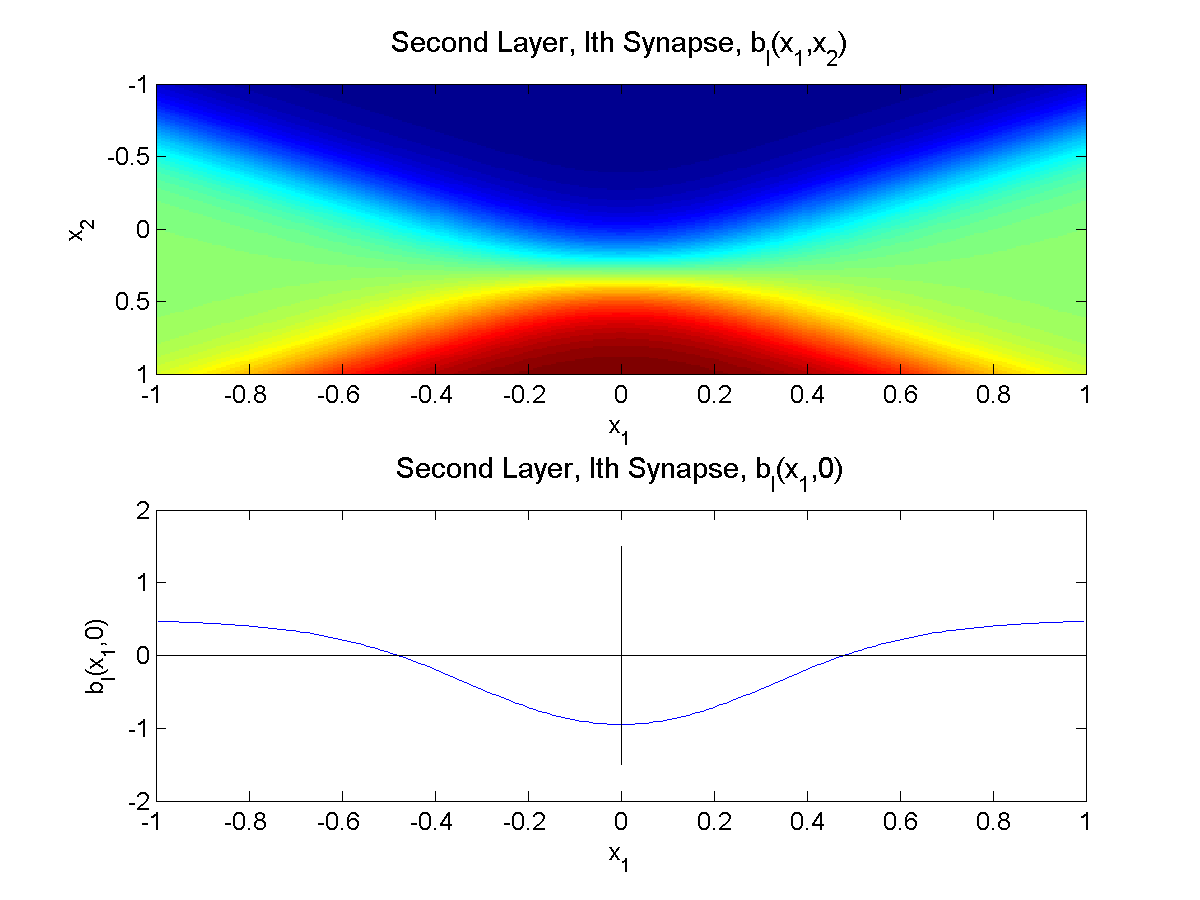
\includegraphics[width=3in]{figs/nn_synapse2.png}}
\end{frame}

\begin{frame}
  \frametitle{Excitation, First Layer:
    $e_k^{(1)}=b_{k}^{(1)}+\sum_{j=1}^2 w_{kj}^{(1)}x_j$} The first
  layer of the neural net just computes a linear function of
  $\vec{x}$. Here's an example:
  \centerline{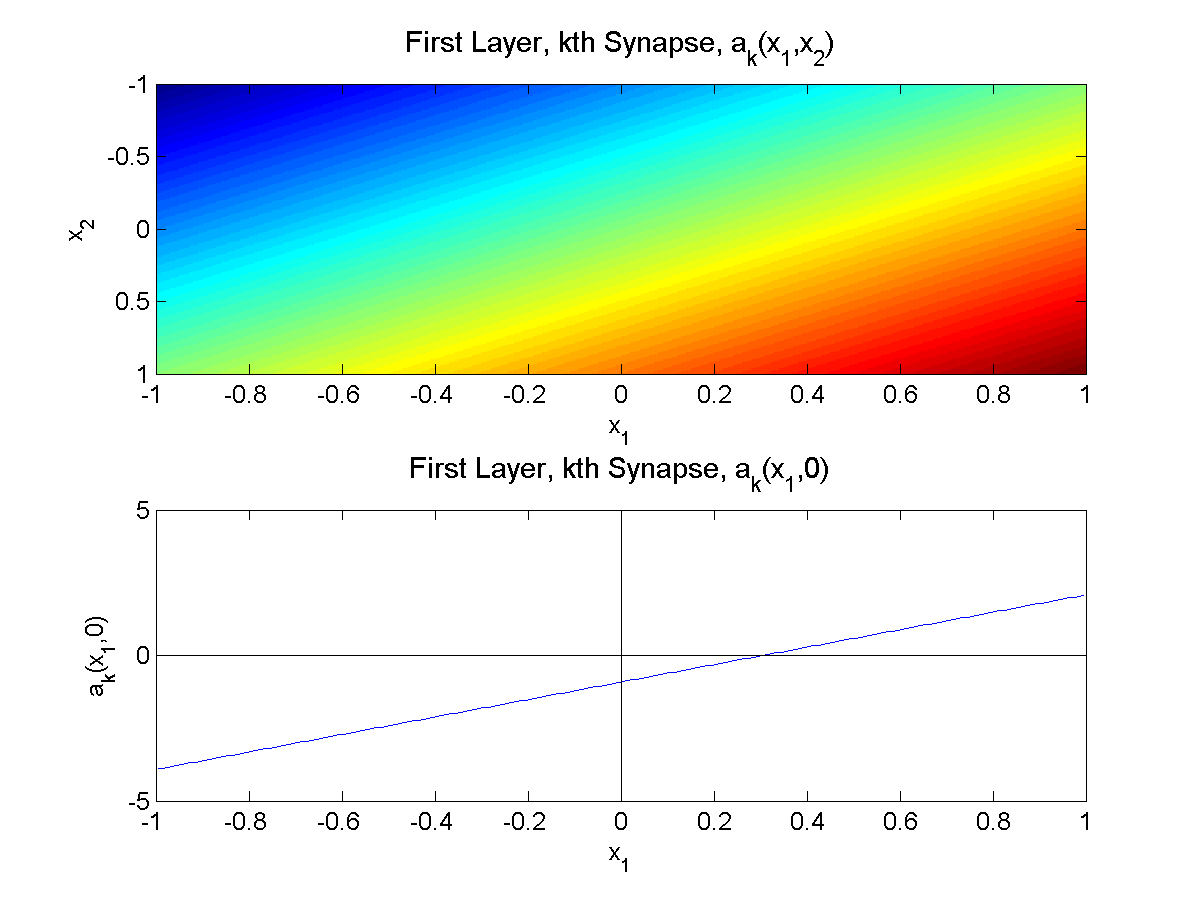
\includegraphics[width=3in]{figs/nn_synapse1.png}}
\end{frame}

\begin{frame}
  \frametitle{Activation, First Layer: $h_k=\tanh(e_k^{(1)})$} The
  activation nonlinearity then ``squashes'' the linear function:
  \centerline{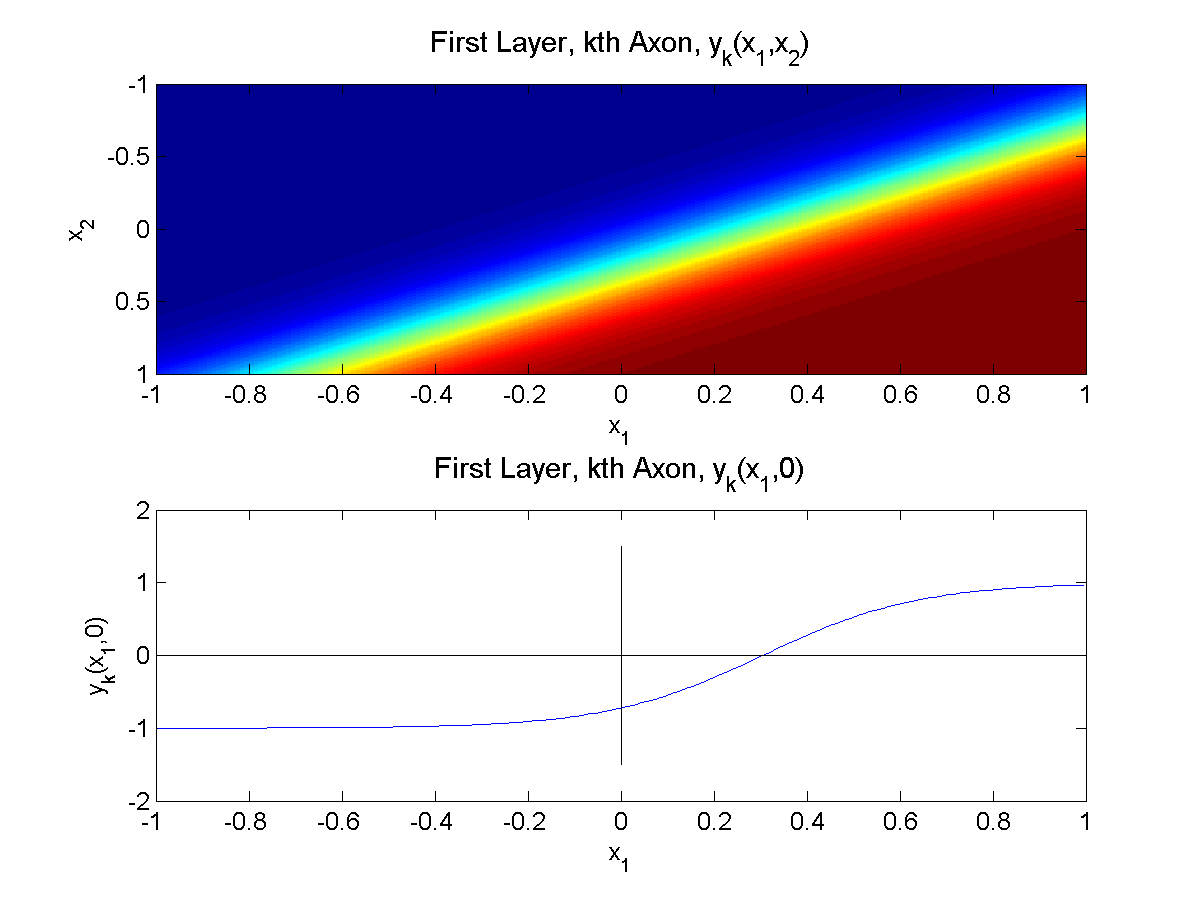
\includegraphics[width=3in]{figs/nn_axon1.png}}
\end{frame}

\begin{frame}
  \frametitle{Second Layer:
    $\hat{y}_k=b_{k}^{(2)}+\sum_{j=1}^2w_{kj}^{(2)}h_k$} The second
  layer then computes a linear combination of the first-layer
  activations, which is sufficient to match our desired function:
  \centerline{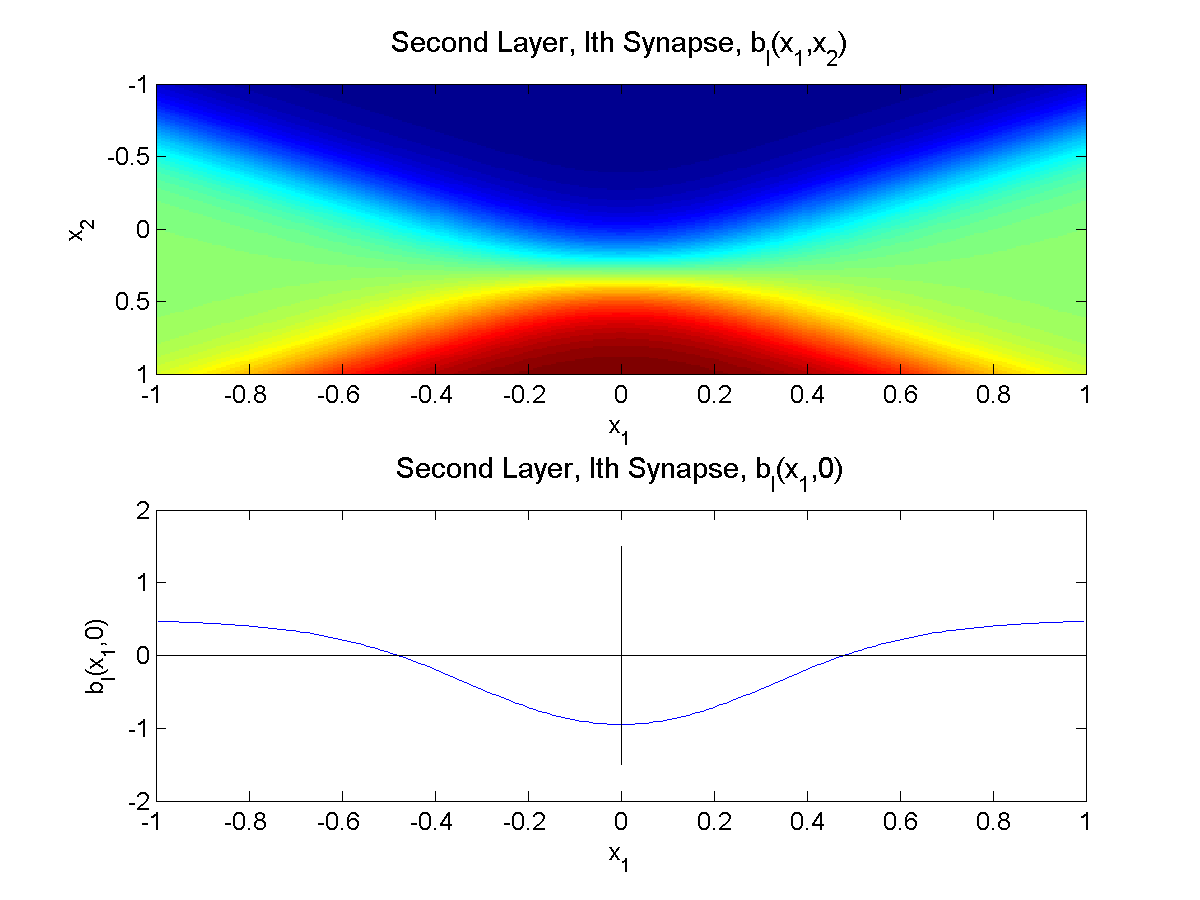
\includegraphics[width=3in]{figs/nn_synapse2.png}}
\end{frame}
%


%%%%%%%%%%%%%%%%%%%%%%%%%%%%%%%%%%%%%%%%%%%%
\section{Binary Nonlinearities}
\setcounter{subsection}{1}

\begin{frame}
  \begin{columns}[t]
    \column{1.85in}
    \begin{block}{The Basic Binary  Nonlinearity: Unit Step (a.k.a. Heaviside function)}
      \[
      u\left(\bar{w}_k^{(1)}\vec{x}\right)=\begin{cases}
      1 & \bar{w}_k^{(1)}\vec{x} > 0\\
      0 & \bar{w}_k^{(1)}\vec{x} < 0
      \end{cases}
      \]
      \centerline{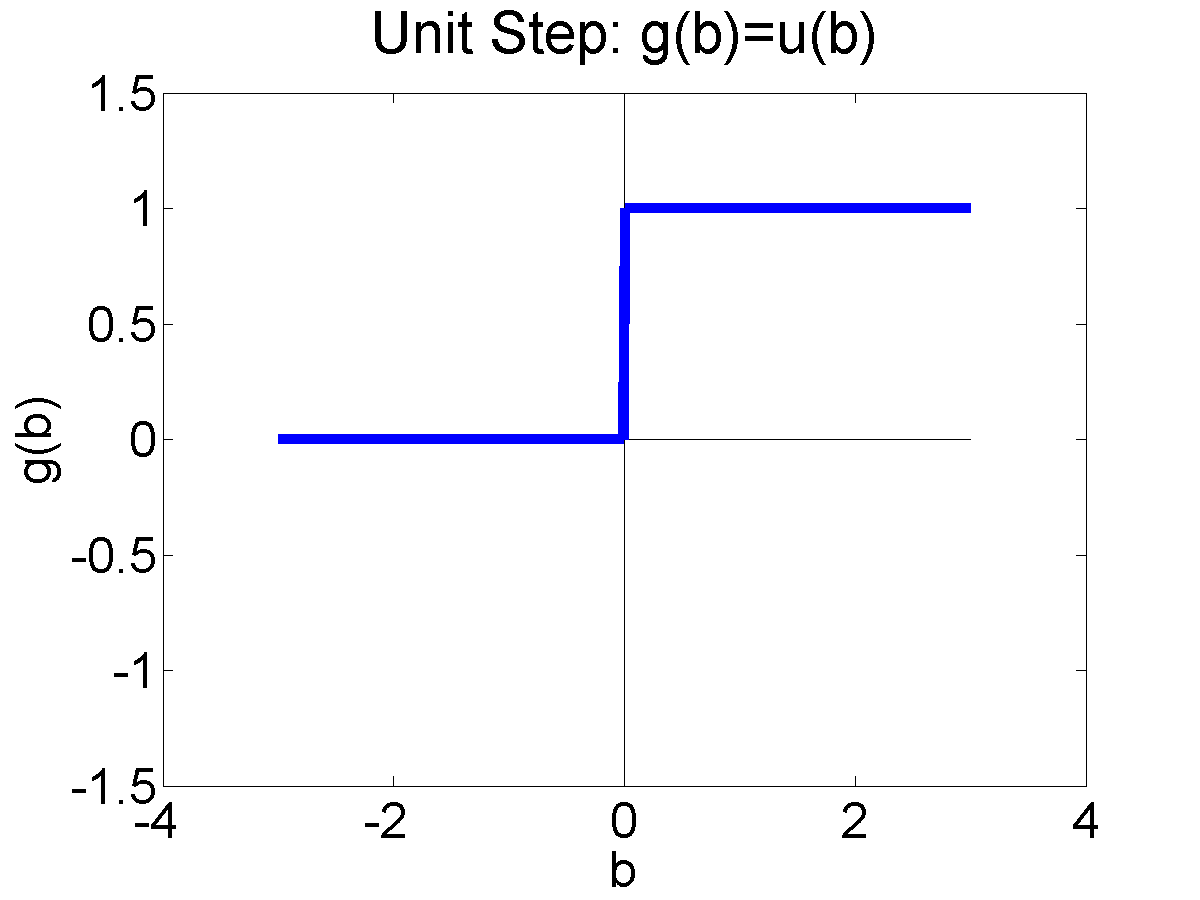
\includegraphics[width=1.75in]{figs/nn_unitstep.png}}
    \end{block}
    \column{2.65in}
    \begin{block}{Pros and Cons of the Unit Step}
      \begin{itemize}
      \item {\bf Pro:} it gives exactly piece-wise constant
        approximation of any desired $\vec{y}$.
      \item {\bf Con:} if $h_k=u(e_k)$, then you can't use
        back-propagation to train the neural network.
      \end{itemize}
      Remember back-prop:
      \[
      \frac{d{\mathcal L}}{dw_{kj}}=
      \sum_k\left(\frac{d{\mathcal L}}{dh_k}\right)
      \left(\frac{\partial h_k}{\partial e_k}\right)
      \left(\frac{\partial e_k}{\partial w_{kj}}\right)
      \]
      but $du(x)/dx$ is a Dirac delta function ---
      zero everywhere, except where it's infinite.
    \end{block}
  \end{columns}
\end{frame}
  
\begin{frame}
  \begin{columns}[t]
    \column{2.25in}
    \begin{block}{The Differentiable Approximation: Logistic Sigmoid}
      \[
      \sigma(b)=\frac{1}{1+e^{-b}}
      \]
      \centerline{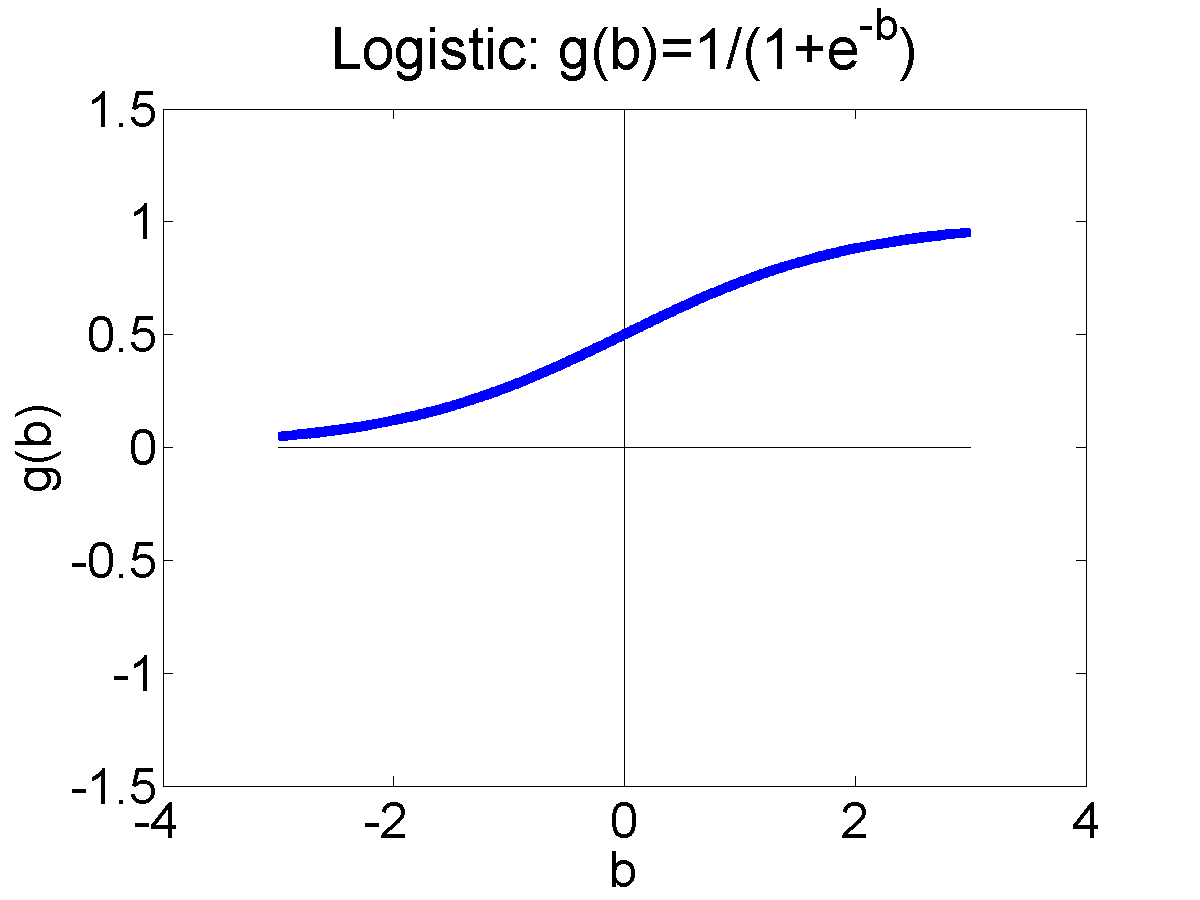
\includegraphics[width=1.75in]{figs/nn_logistic.png}}
    \end{block}
    \column{2.25in}
    \begin{block}{Why to use the logistic function}
      \[
      \sigma(b) = \begin{cases}
        1 & b\rightarrow\infty\\
        0 & b\rightarrow -\infty\\
        \mbox{in between} & \mbox{in between}
      \end{cases}
      \]
      and $\sigma(b)$ is smoothly differentiable, so
      back-prop works.
    \end{block}
  \end{columns}
\end{frame}

\begin{frame}
  \frametitle{Derivative of a sigmoid}
  The derivative of a sigmoid is pretty easy to calculate:
  \[
  \sigma(x)=\frac{1}{1+e^{-x}},~~~\frac{d\sigma}{dx}=\frac{e^{-x}}{(1+e^{-x})^2}
  \]
  An interesting fact that's extremely useful, in computing back-prop,
  is that if $h=\sigma(x)$, then we can write the derivative in terms
  of $h$, without any need to store $x$:
  \begin{align*}
    \frac{d\sigma}{dx} &=\frac{e^{-x}}{(1+e^{-x})^2}\\
    &=\left(\frac{1}{1+e^{-x}}\right)\left(\frac{e^{-x}}{1+e^{-x}}\right)\\
    &=\left(\frac{1}{1+e^{-x}}\right)\left(1-\frac{1}{1+e^{-x}}\right)\\
    &=\sigma(x)(1-\sigma(x))\\
    &=h(1-h)\\
  \end{align*}
\end{frame}

\begin{frame}
  \begin{columns}[t]
    \column{2.25in}
    \begin{block}{Step function and its derivative}
      \centerline{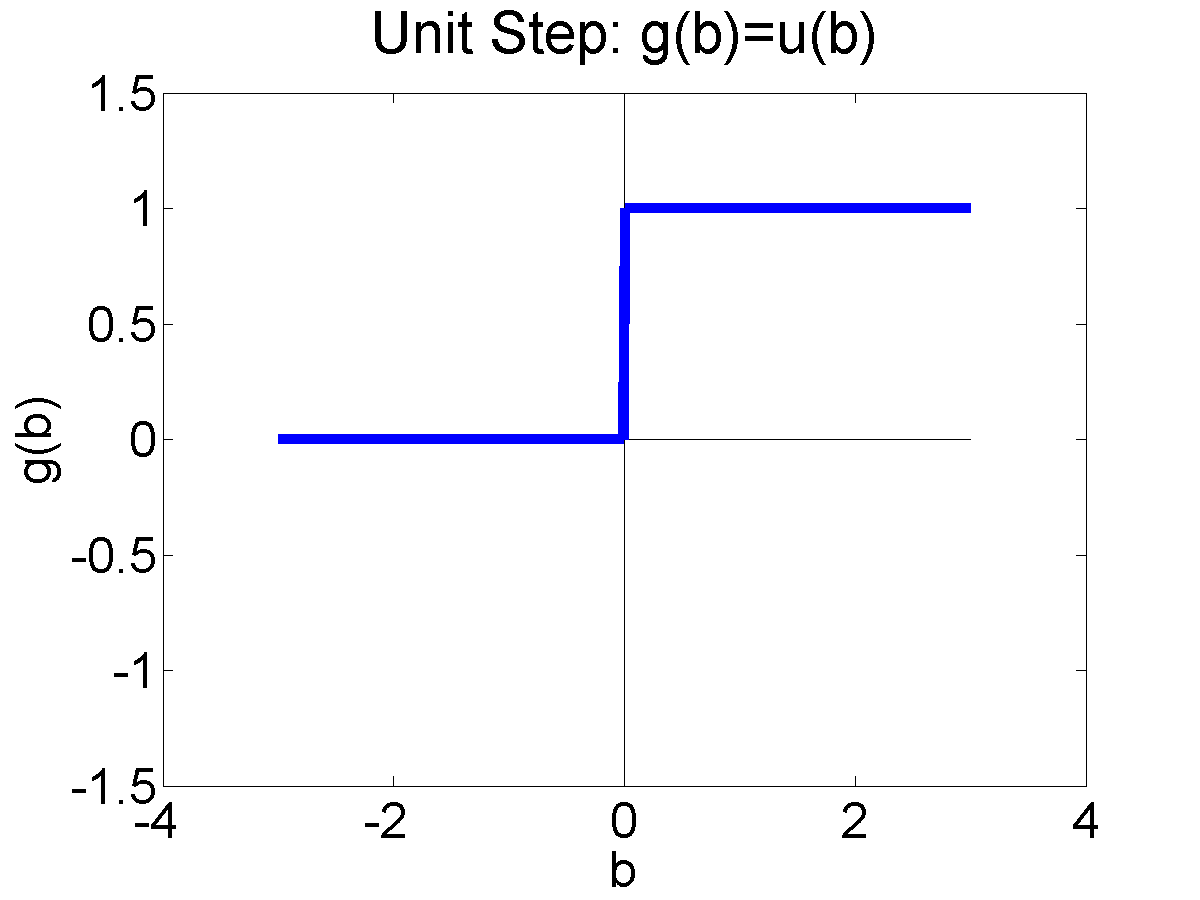
\includegraphics[width=1.75in]{figs/nn_unitstep.png}}
      \begin{itemize}
      \item The derivative of the step function is the Dirac
        delta, which is not very useful in backprop.
      \end{itemize}
    \end{block}
    \column{2.25in}
    \begin{block}{Logistic function and its derivative}
      \centerline{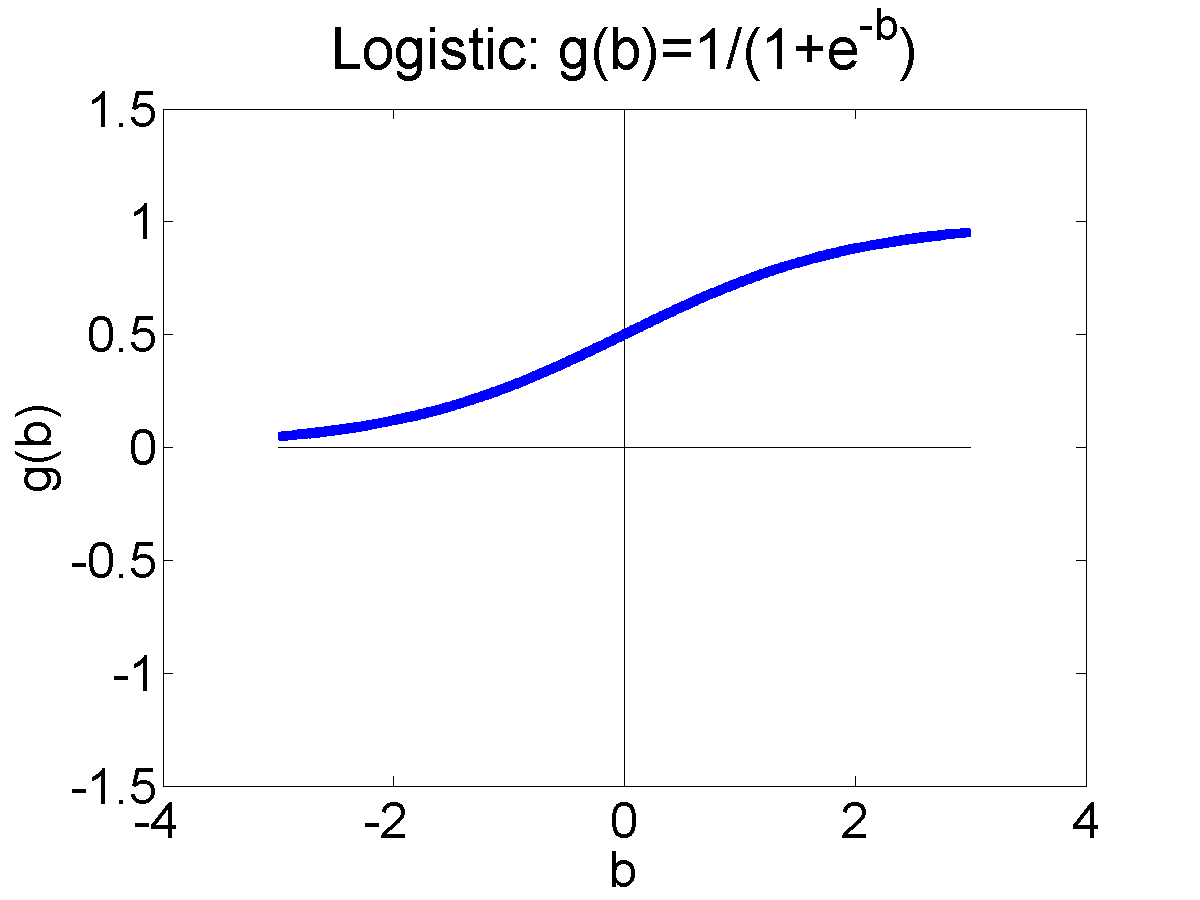
\includegraphics[width=1.75in]{figs/nn_logistic.png}}
      \centerline{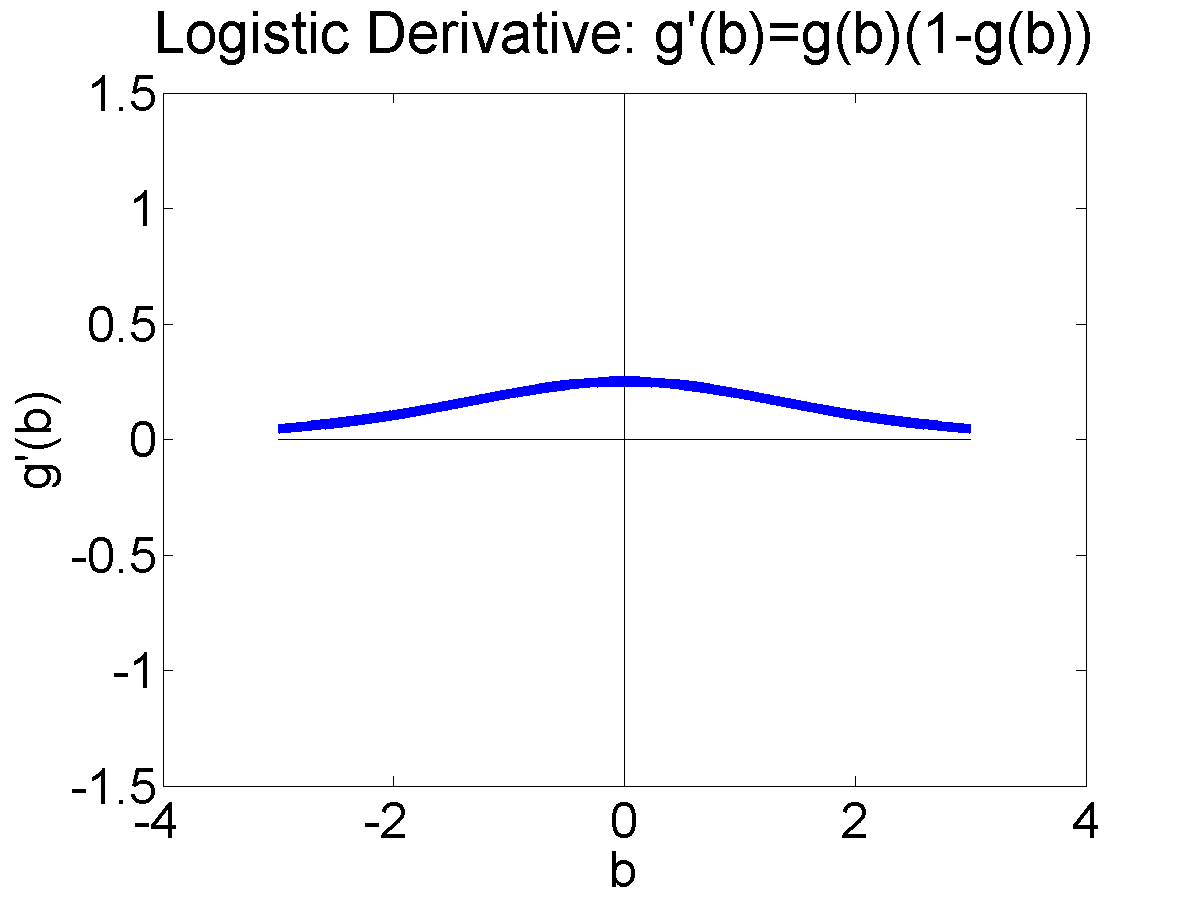
\includegraphics[width=1.75in]{figs/nn_logisticprime.png}}
    \end{block}
  \end{columns}
\end{frame}

\begin{frame}
  \frametitle{Signum and Tanh}

  The signum function is a signed binary nonlinearity.  It is used if,
  for some reason, you want your output to be
  $h\in\left\{-1,1\right\}$, instead of $h\in\left\{0,1\right\}$:
  \[
  \mbox{sign}(b)=\begin{cases}
  -1 & b<0\\
  1 & b>0
  \end{cases}
  \]
  It is usually approximated by the hyperbolic tangent function
  (tanh), which is just a scaled shifted version of the sigmoid:
  \begin{displaymath}
    \tanh(b) = \frac{e^b-e^{-b}}{e^b+e^{-b}}
    = \frac{1-e^{-2b}}{1+e^{-2b}}
    = 2\sigma(2b)-1
  \end{displaymath}
  and which has a scaled version of the sigmoid derivative:
  \begin{align*}
    \frac{d\tanh(b)}{db} =\left(1-\tanh^2(b)\right)
  \end{align*}
\end{frame}

\begin{frame}
  \begin{columns}[t]
    \column{2.25in}
    \begin{block}{Signum function and its derivative}
      \centerline{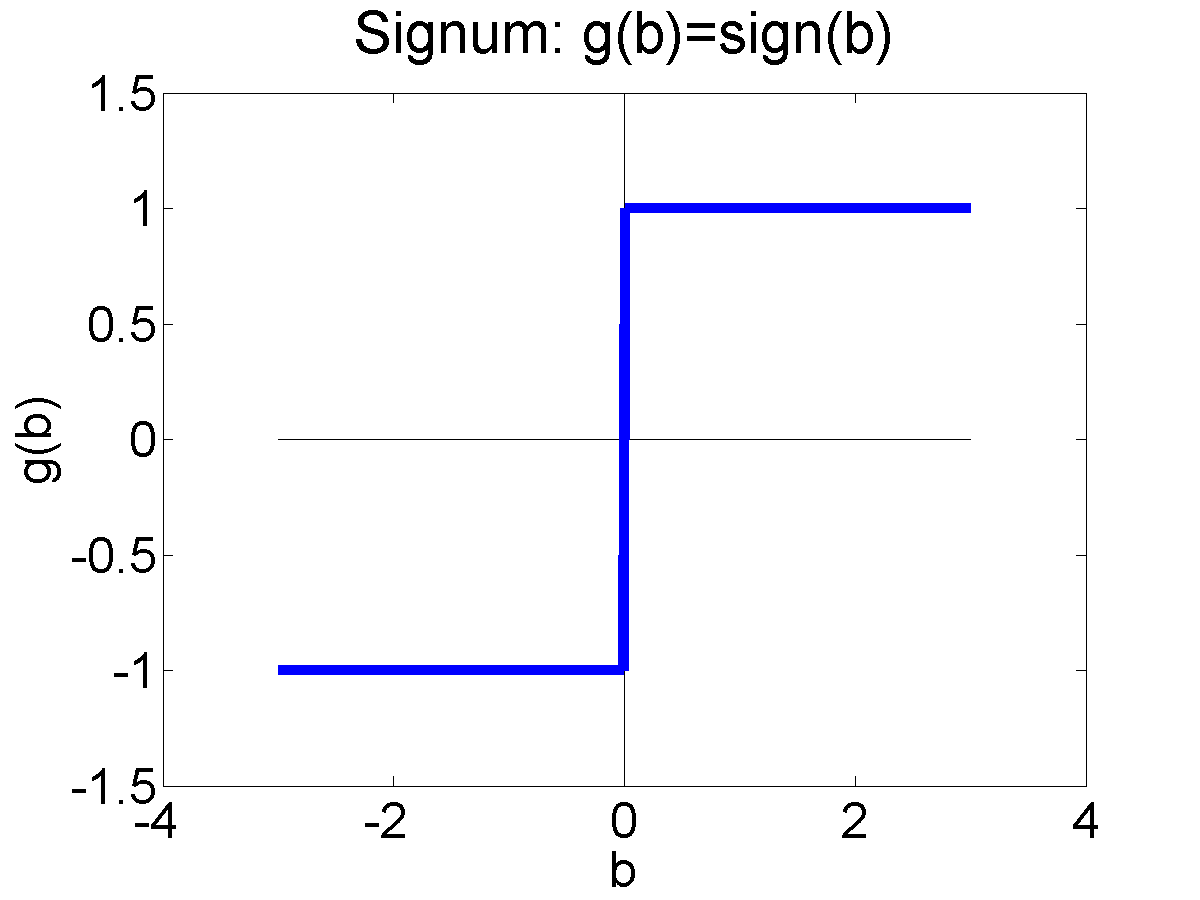
\includegraphics[width=1.75in]{figs/nn_signum.png}}
      \begin{itemize}
      \item The derivative of the signum function is the Dirac
        delta, which is not very useful in backprop.
      \end{itemize}
    \end{block}
    \column{2.25in}
    \begin{block}{Tanh function and its derivative}
      \centerline{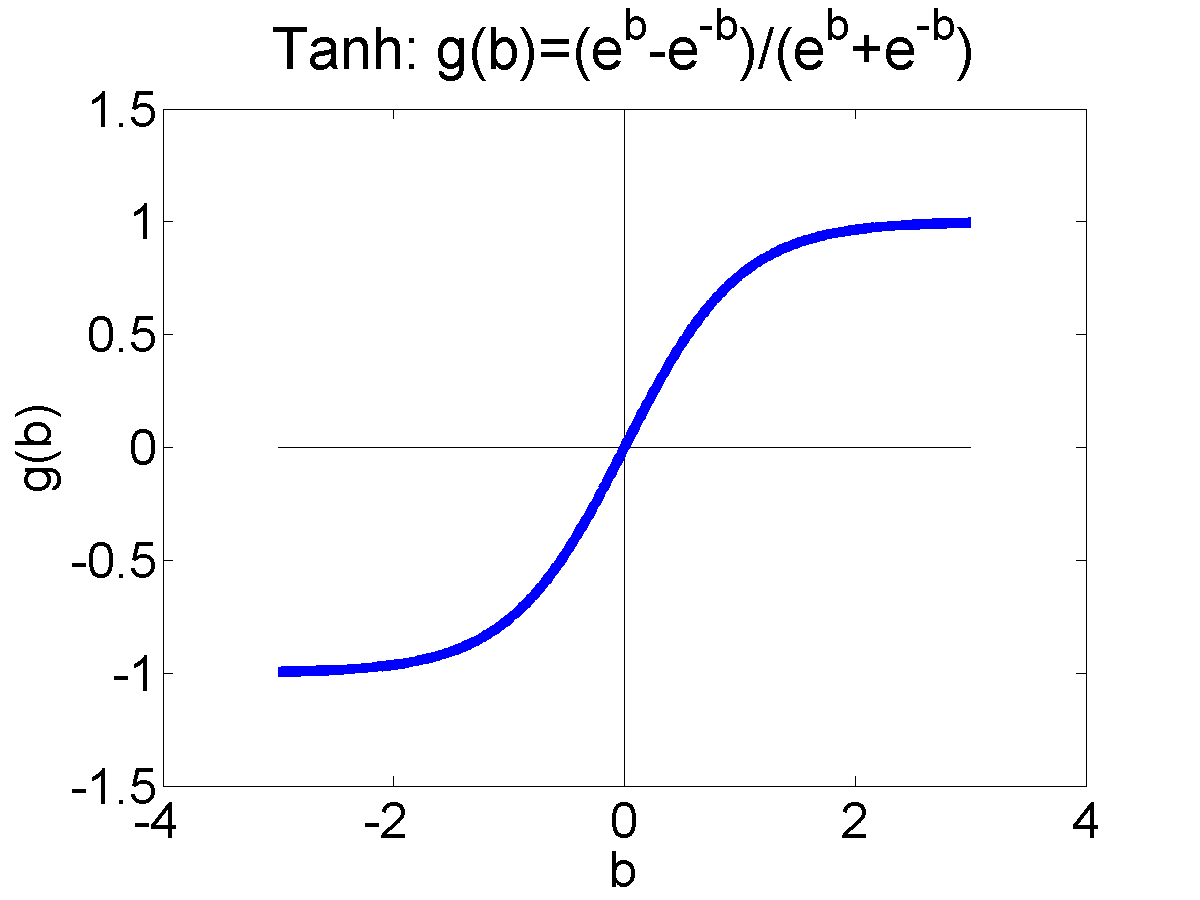
\includegraphics[width=1.75in]{figs/nn_tanh.png}}
      \centerline{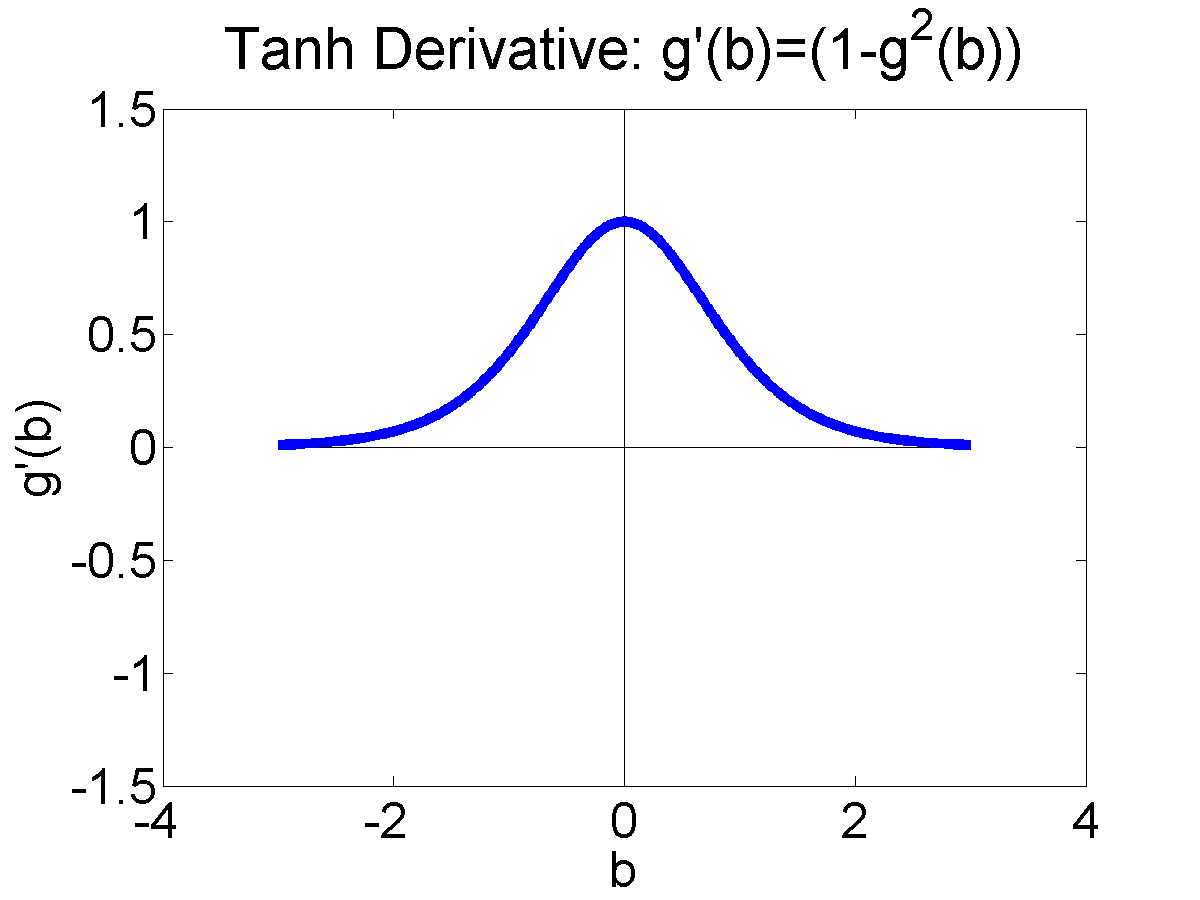
\includegraphics[width=1.75in]{figs/nn_tanhprime.png}}
    \end{block}
  \end{columns}
\end{frame}

\begin{frame}
  \frametitle{A suprising problem with the sigmoid: Vanishing gradients}
  \centerline{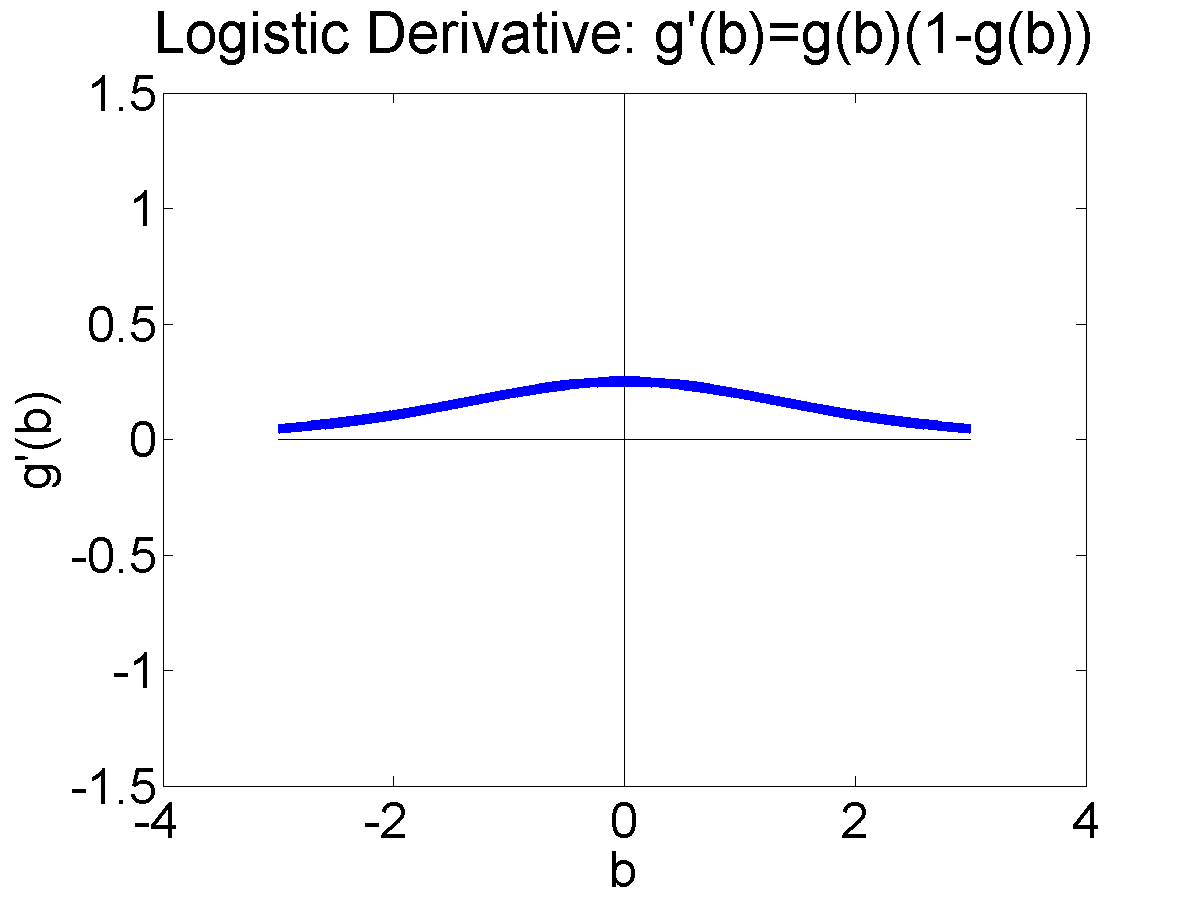
\includegraphics[width=1in]{figs/nn_logisticprime.png}}
  
  The sigmoid has a surprising problem: for large values of $w$,
  $\sigma'(wx)\rightarrow 0$.
  \begin{itemize}
  \item When we begin training, we start with small values of $w$.
    $\sigma'(wx)$ is reasonably large, and training proceeds.
  \item If $w$ and $\nabla_{w}{\mathcal L}$ are vectors in opposite
    directions, then $w\leftarrow w-\eta\nabla_{w}{\mathcal L}$ makes
    $w$ larger.  After a few iterations, $w$ gets very large.  At that
    point, $\sigma'(wx)\rightarrow 0$, and training effectively stops.
  \item After that point, even if the neural net sees new training
    data that don't match what it has already learned, it can no
    longer change.  We say that it has suffered from the ``vanishing
    gradient problem.''
  \end{itemize}
\end{frame}
    
\begin{frame}
  \frametitle{A solution to the vanishing gradient problem: ReLU}
  \centerline{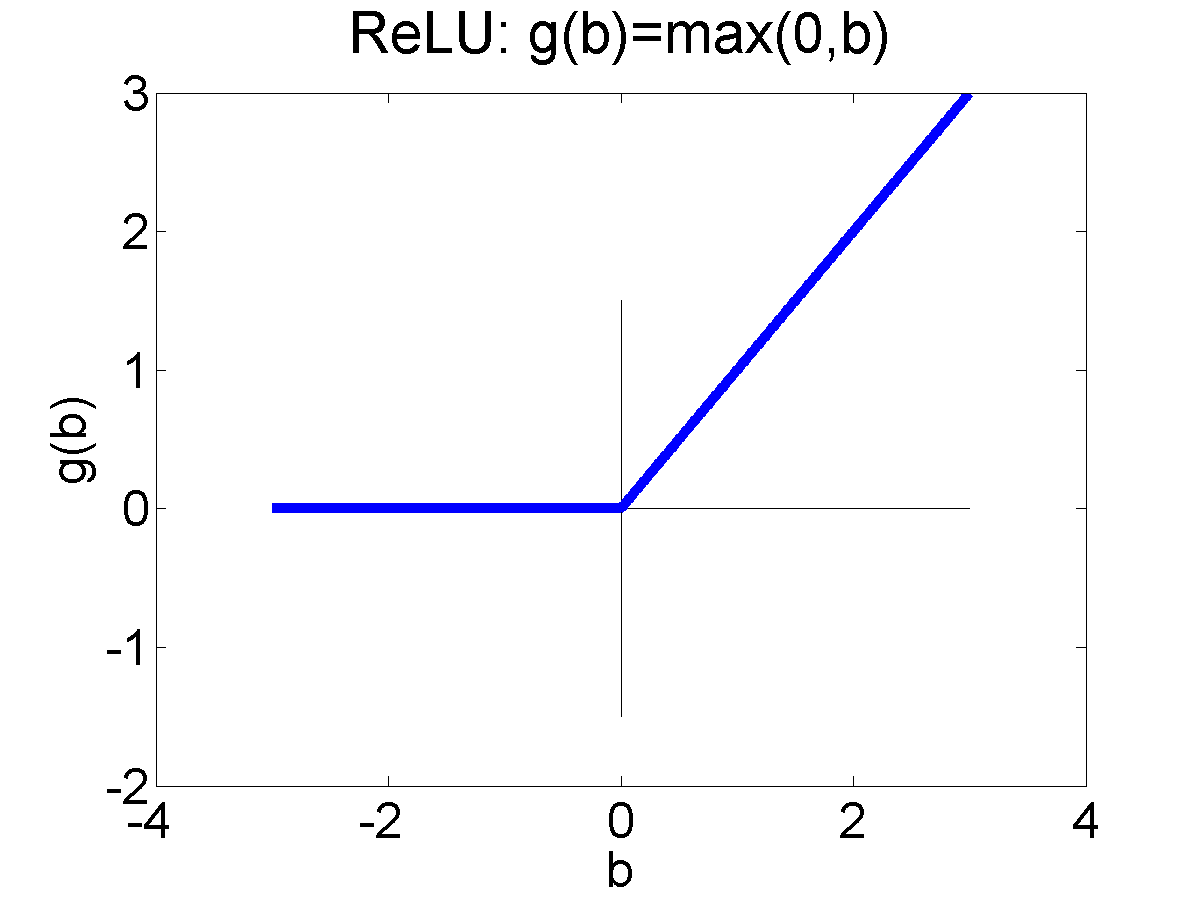
\includegraphics[width=1in]{figs/nn_relu.png}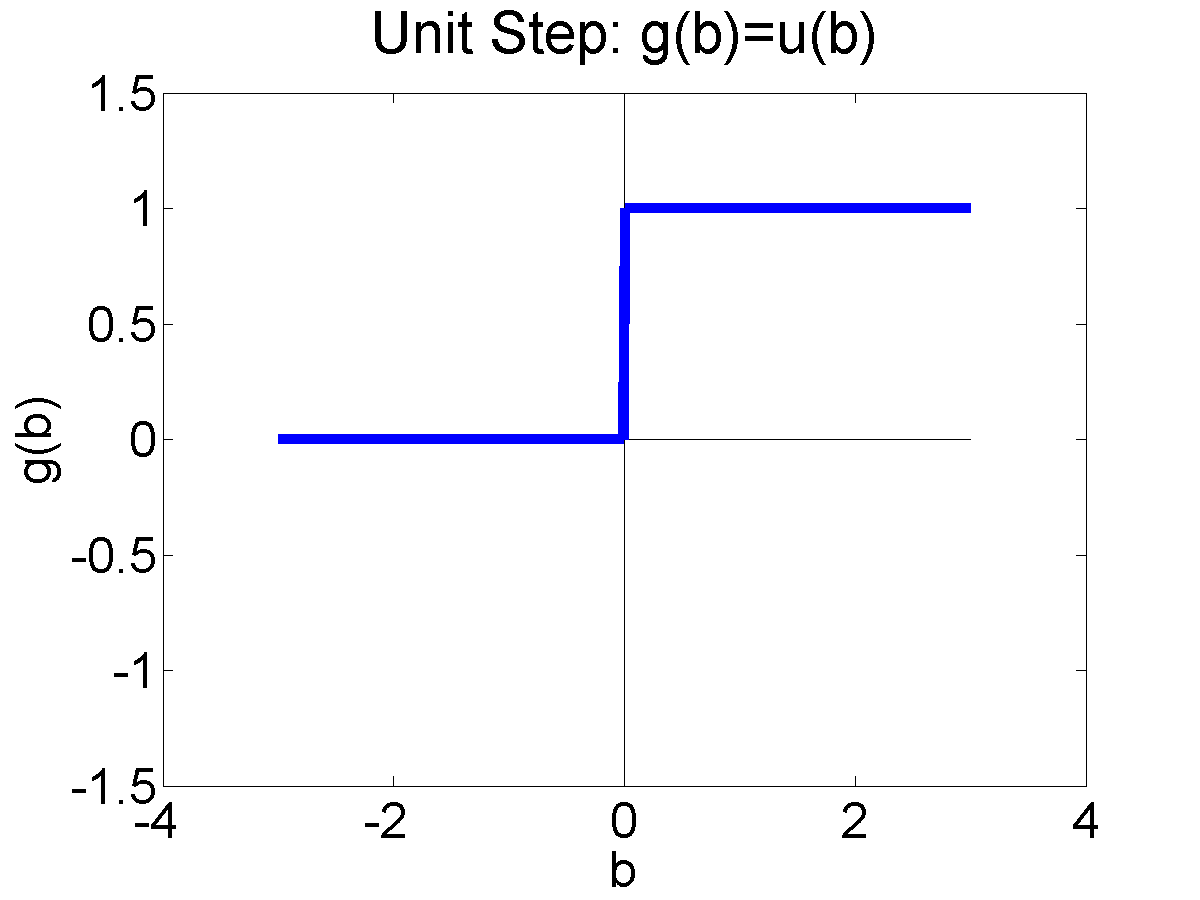
\includegraphics[width=1in]{figs/nn_unitstep.png}}

  The most ubiquitous solution to the vanishing gradient problem is to
  use a ReLU (rectified linear unit) instead of a sigmoid.  The ReLU
  is given by
  \[
  \mbox{ReLU}(b) = \begin{cases}
    b & b\ge 0\\
    0 & b\le 0,
  \end{cases}
  \]
  and its derivative is the unit step.  Notice that the
  unit step is equally large ($u(wx)=1$)  for any positive value ($wx>0$), so
  no matter how large $w$ gets, back-propagation continues to work.
\end{frame}

\begin{frame}
  \frametitle{A solution to the vanishing gradient problem: ReLU}
  \centerline{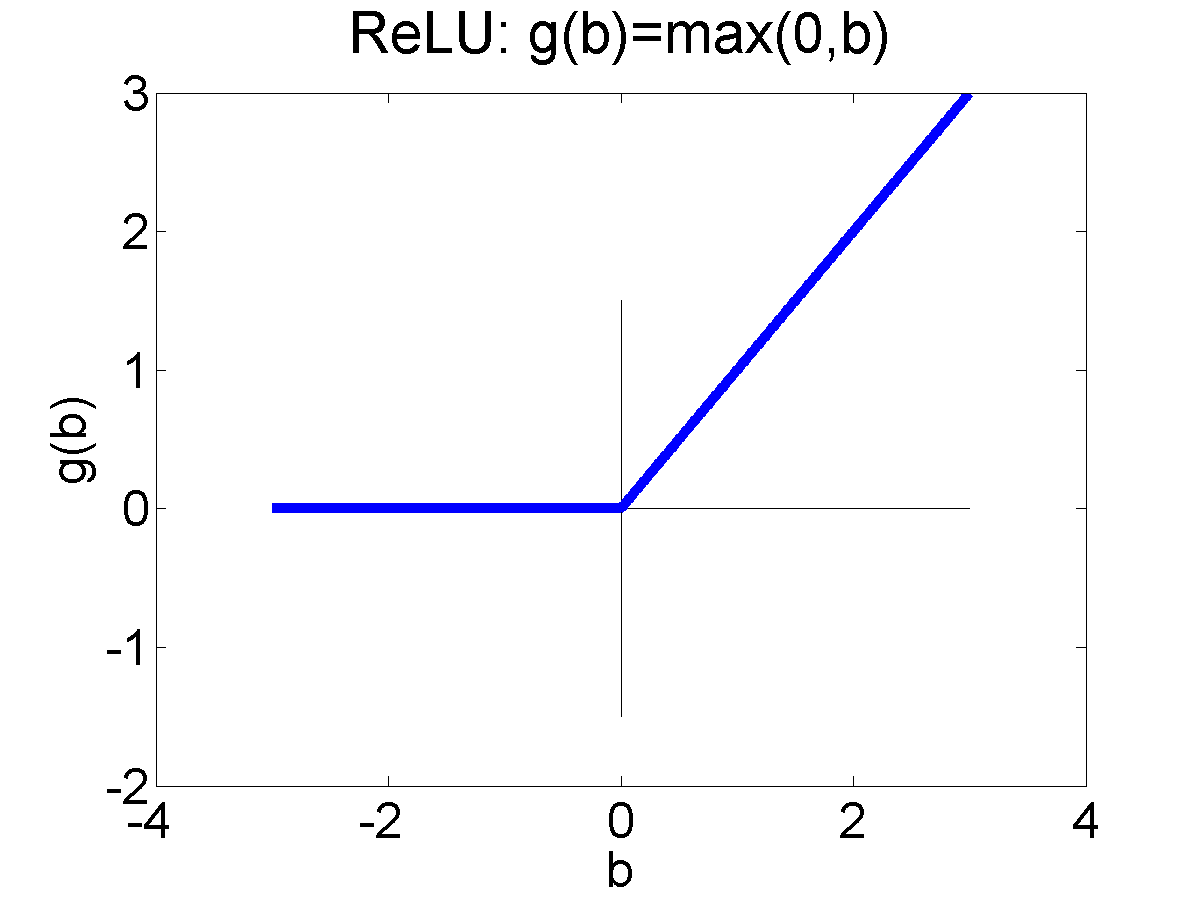
\includegraphics[width=1in]{figs/nn_relu.png}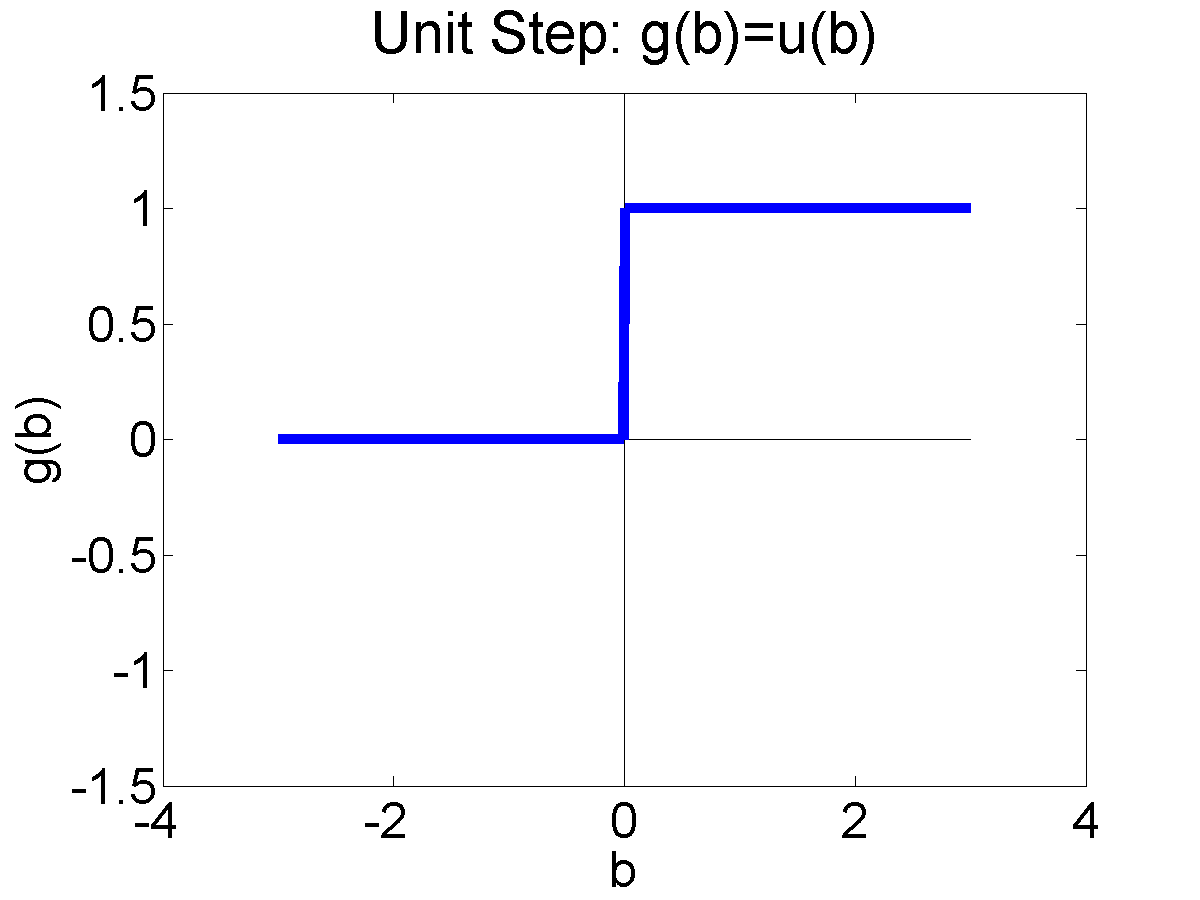
\includegraphics[width=1in]{figs/nn_unitstep.png}}

  \begin{itemize}
    \item {\bf Pro:} The ReLU derivative is equally large
      ($\frac{d\mbox{ReLU}(wx)}{d(wx)}=1$) for any positive value
      ($wx>0$), so no matter how large $w$ gets, back-propagation
      continues to work.
    \item {\bf Con:} If the ReLU is used as a hidden unit
      ($h_j=\mbox{ReLU}(e_j)$), then your output is no longer a
      piece-wise constant approximation of $\vec{y}$.  It is now
      piece-wise linear.
    \item On the other hand, maybe piece-wise linear is
      better than piece-wise constant, so\ldots
  \end{itemize}
\end{frame}
      
\begin{frame}
  \frametitle{A solution to the vanishing gradient problem: the ReLU}
  \centerline{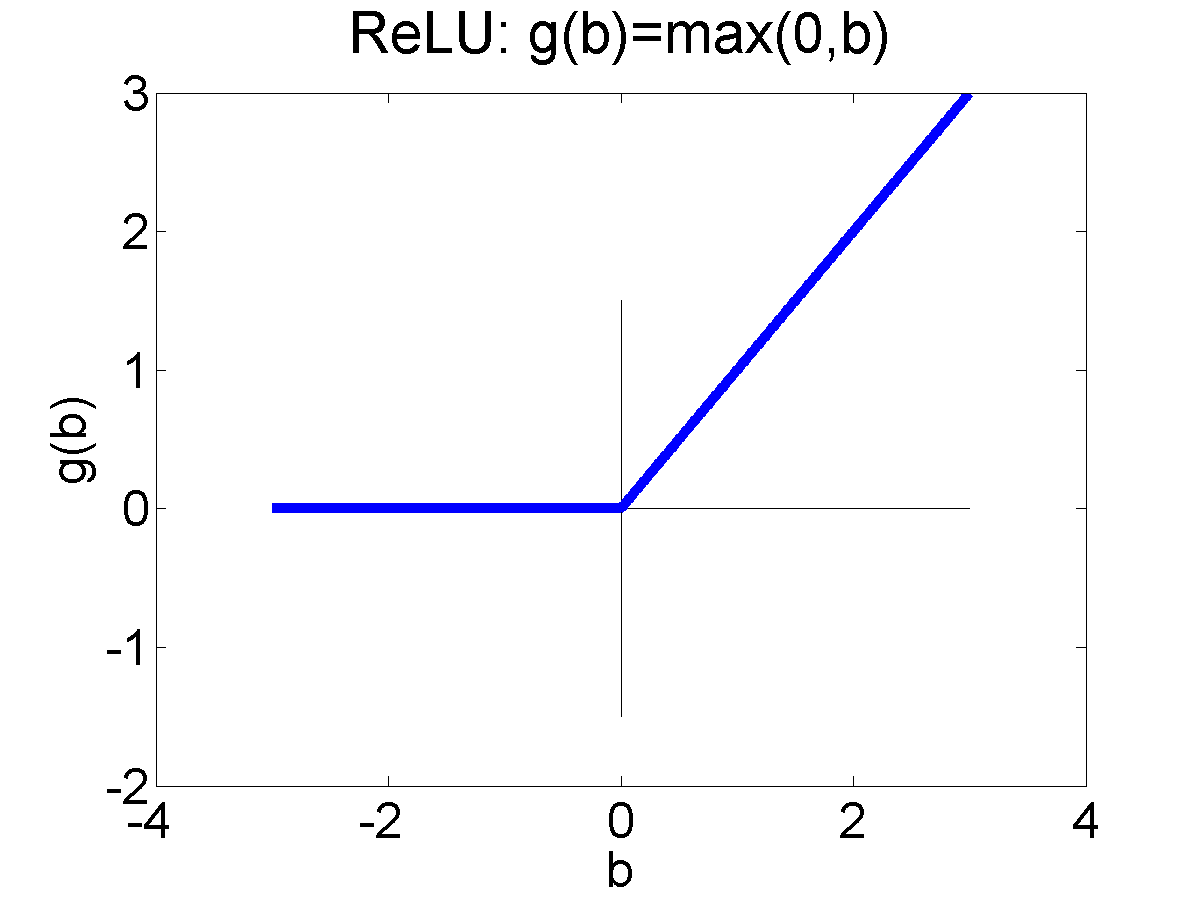
\includegraphics[width=1in]{figs/nn_relu.png}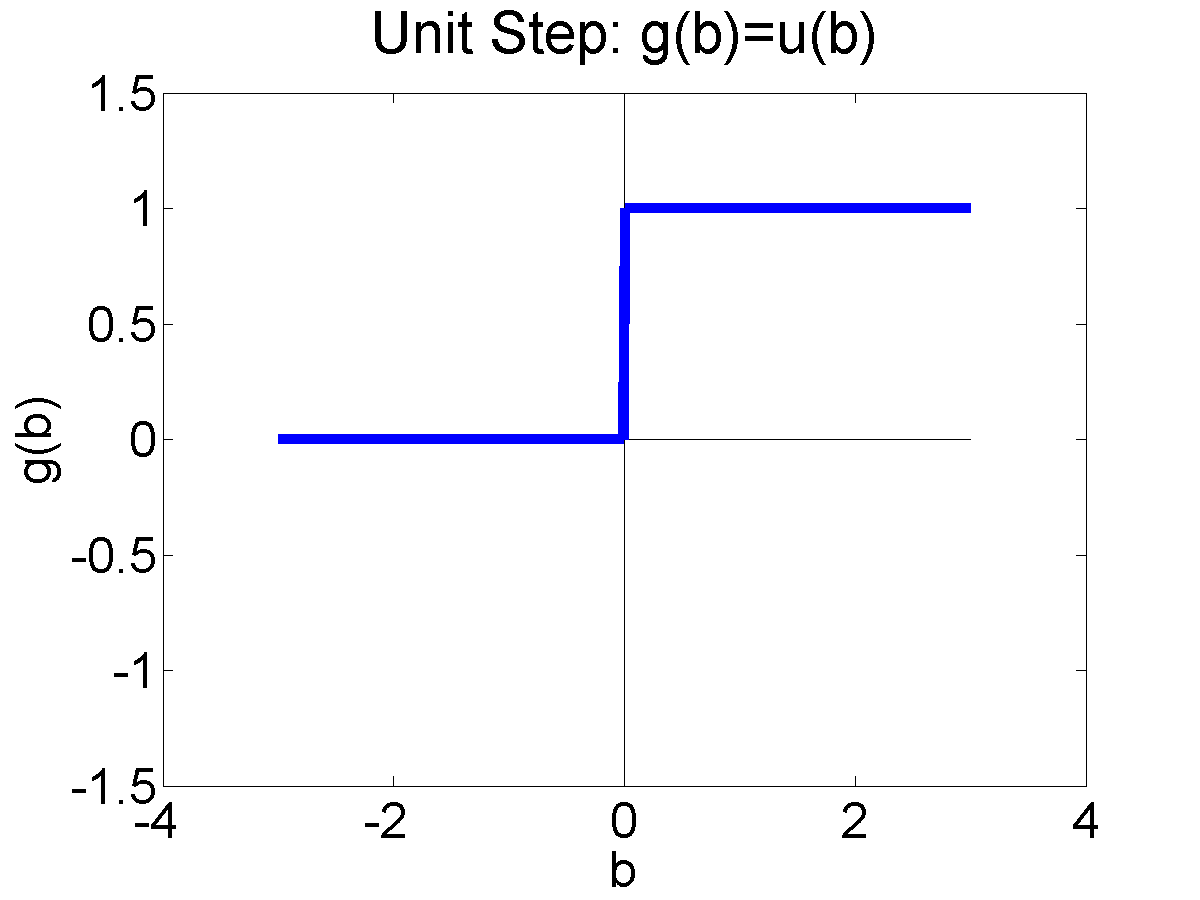
\includegraphics[width=1in]{figs/nn_unitstep.png}}

  \begin{itemize}
    \item {\bf Pro:} The ReLU derivative is equally large
      ($\frac{d\mbox{ReLU}(wx)}{d(wx)}=1$) for any positive value
      ($wx>0$), so no matter how large $w$ gets, back-propagation
      continues to work.
    \item {\bf Pro:} If the ReLU is used as a hidden unit
      ($h_j=\mbox{ReLU}(e_j)$), then your output is no longer a
      piece-wise constant approximation of $\vec{y}$.  It is now
      piece-wise linear.
    \item {\bf Con:} ??
  \end{itemize}
\end{frame}

\begin{frame}
  \frametitle{The dying ReLU problem}
  \centerline{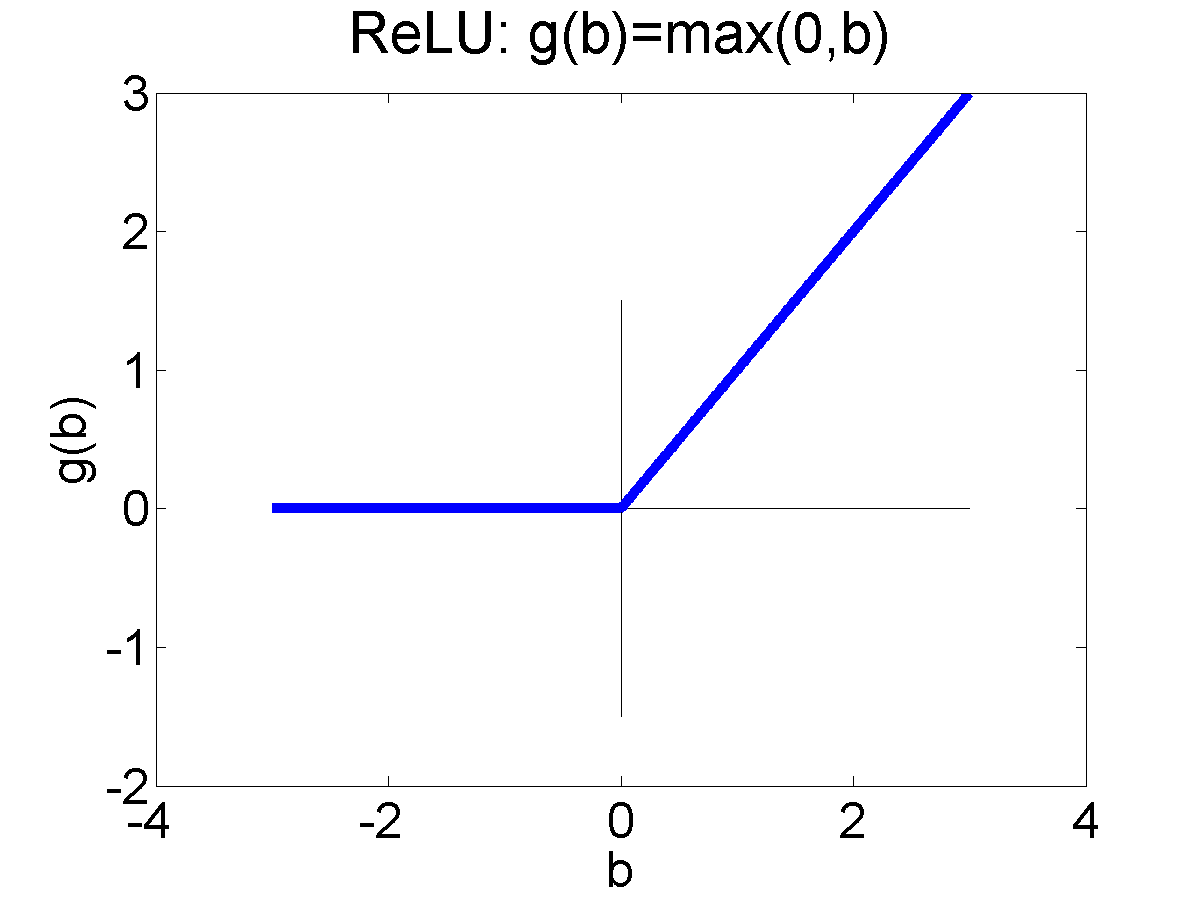
\includegraphics[width=1in]{figs/nn_relu.png}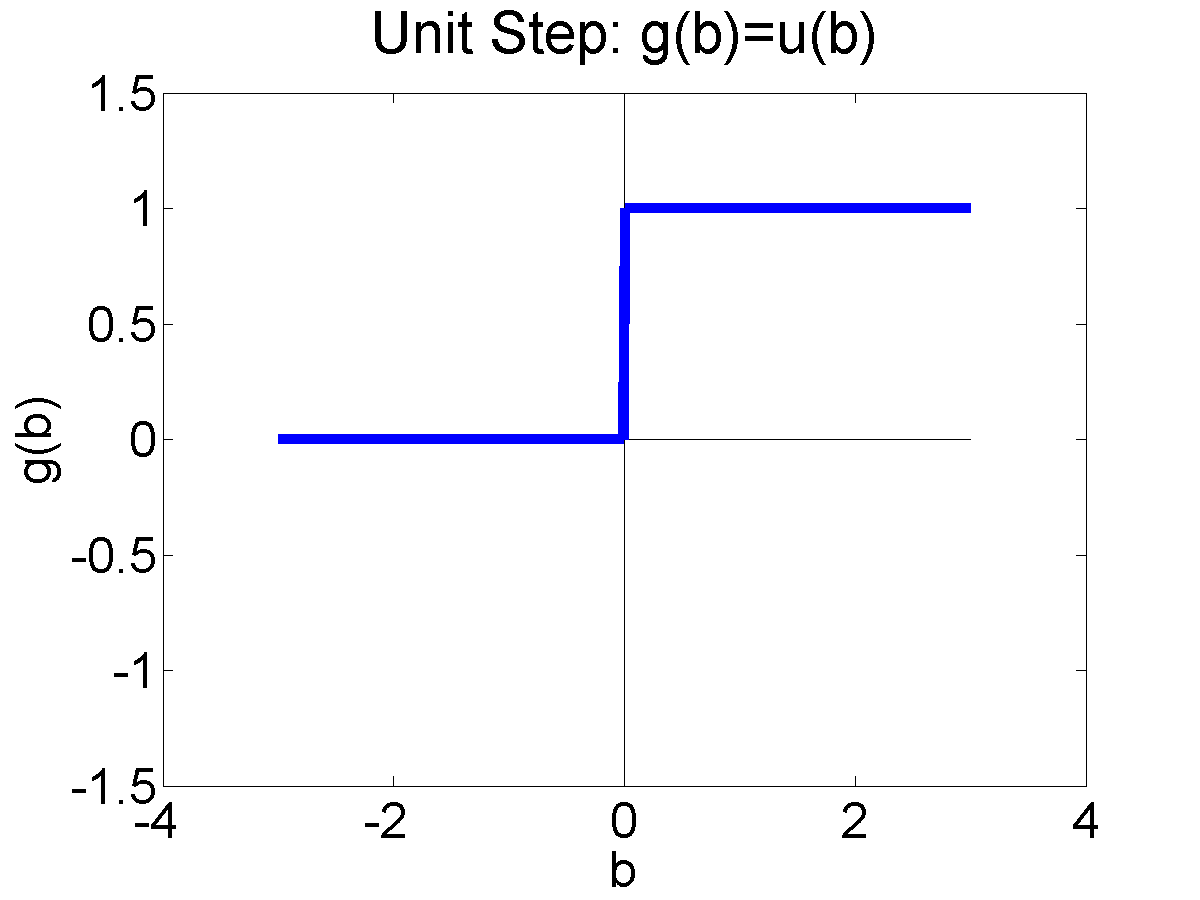
\includegraphics[width=1in]{figs/nn_unitstep.png}}

  \begin{itemize}
    \item {\bf Pro:} The ReLU derivative is equally large
      ($\frac{d\mbox{ReLU}(wx)}{d(wx)}=1$) for any positive value
      ($wx>0$), so no matter how large $w$ gets, back-propagation
      continues to work.
    \item {\bf Pro:} If the ReLU is used as a hidden unit
      ($h_j=\mbox{ReLU}(e_j)$), then your output is no longer a
      piece-wise constant approximation of $\vec{y}$.  It is now
      piece-wise linear.
    \item {\bf Con:} If $wx+b<0$, then
      ($\frac{d\mbox{ReLU}(wx)}{d(wx)}=0$), and learning stops.
      In the worst case, if $b$ becomes very negative, then all of the
      hidden nodes are turned off---the network computes nothing, and
      no learning can take place!  This is called the ``Dying ReLU
      problem.''
  \end{itemize}
\end{frame}

\begin{frame}
  \frametitle{Solutions to the Dying ReLU problem}

  \begin{itemize}
  \item {\bf Softplus:}  Pro: always positive.  Con: gradient$\rightarrow 0$ as $x\rightarrow -\infty$.
    \[
    f(x) = \ln\left(1+e^x\right)
    \]
  \item {\bf Leaky ReLU:} Pro: gradient constant, output piece-wise linear.  Con:
    negative part might fail to match your dataset.
    \[
    f(x) = \begin{cases}
      x & x \ge 0\\
      0.01x & x \le 0
    \end{cases}
    \]
  \item {\bf Parametric ReLU (PReLU:)} Pro: gradient constant, ouput
    PWL.  The slope of the negative part ($a$) is a trainable
    parameter, so can adapt to your dataset.  Con: you have to train it.
    \[
    f(x) = \begin{cases}
      x & x \ge 0\\
      ax & x \le 0
    \end{cases}
    \]
  \end{itemize}
\end{frame}

%%%%%%%%%%%%%%%%%%%%%%%%%%%%%%%%%%%%%%%%%%%%%%%%%%%%%%%%%%%%%%%
\section[Example \#2]{Example \#2: Semicircle $\rightarrow$ Parabola}
\setcounter{subsection}{1}

\begin{frame}
  \frametitle{Example \#2: Semicircle $\rightarrow$ Parabola}

  Can we design a neural net that converts a semicircle
  ($x_0^2+x_1^2=1$) to a parabola ($y_1=y_0^2$)?
  \centerline{\includegraphics[height=2in]{exp/nn_target_figure.png}}
\end{frame}

\begin{frame}
  \frametitle{Two-Layer Feedforward Neural Network}
  \begin{small}\begin{center}
  \tikzstyle{pre}=[<-,shorten <=1pt,>=stealth',semithick,draw=blue]
  \tikzstyle{post}=[->,shorten >=1pt,>=stealth',semithick,draw=blue]
  \begin{tikzpicture}[
      open/.style={circle,thick, draw=blue, text=black, align=left, text width=0.5cm}
    ]
    \node (x0) at (0,0.25) {$1$};
    \node[open] (x1) at (1,0) {$x_1$};
    \node[open] (x2) at (2,0) {$x_2$};
    \node (x3) at (2.75,0) {\ldots};
    \node[open] (xm0) at (3.5,0) {$x_{m_0}$};
    \node (input) at (6,0) {$\mathbf{a}_0=\mathbf{x}$ is the input vector};
    \node[open] (z11) at (1,1.3) {$z_{1,1}$} edge[pre](x0) edge[pre](x1) edge[pre](x2) edge[pre](xm0);
    \node[open] (z12) at (2,1.3) {$z_{1,2}$} edge[pre](x0) edge[pre](x1) edge[pre](x2) edge[pre](xm0);
    \node (z13) at (2.75,1.3) {\ldots};
    \node[open] (z1m1) at (3.5,1.3) {$z_{1,m_1}$} edge[pre](x0) edge[pre](x1) edge[pre](x2) edge[pre](xm0);
    \node (z1eq) at (6,1.3) {$\mathbf{z}_1=\mathbf{W}_1\mathbf{x}+\mathbf{b}_1$};
    \node (a10) at (0,2.7) {$1$};
    \node[open] (a11) at (1,2.45) {$a_{1,1}$} edge[pre](z11);
    \node[open] (a12) at (2,2.45) {$a_{1,2}$} edge[pre](z12);
    \node (a13) at (2.75,2.45) {\ldots};
    \node[open] (a1m1) at (3.5,2.45) {$a_{1,m_1}$} edge[pre](z1m1);
    \node (a1eq) at (6,2.45) {$\mathbf{a}_1=\mathbf{f}_1(\mathbf{z}_1)$};
    \node[open] (z21) at (1,3.75) {$z_{2,1}$} edge[pre](a10) edge[pre](a11) edge[pre](a12) edge[pre](a1m1);
    \node[open] (z22) at (2,3.75) {$z_{2,2}$} edge[pre](a10) edge[pre](a11) edge[pre](a12) edge[pre](a1m1);
    \node (z23) at (2.75,3.75) {\ldots};
    \node[open] (z2m2) at (3.5,3.75){$z_{2,m_2}$}edge[pre](a10) edge[pre](a11) edge[pre](a12) edge[pre](a1m1);
    \node (z2eq) at (6,3.75) {$\mathbf{z}_2=\mathbf{W}_2\mathbf{a}_1+\mathbf{b}_2$};
    \node[open] (a21) at (1,4.9) {$g_{1}$} edge[pre](z21);
    \node[open] (a22) at (2,4.9) {$g_{2}$} edge[pre](z22);
    \node (a23) at (2.75,4.9) {\ldots};
    \node[open] (a2m2) at (3.5,4.9) {$g_{m_2}$} edge[pre](z2m2);
    \node (z2eq) at (6,4.9) {$\mathbf{g}(\mathbf{x})=\mathbf{a}_2=\mathbf{f}_2(\mathbf{z}_2)$};
    \node (output) at (2.2,5.65) {${\mathcal{L}}=E\left[-\ln\Pr(\mathbf{y}|\mathbf{g}(\mathbf{x}))\right]$};
  \end{tikzpicture}
\end{center}
\end{small}
\end{frame}

\begin{frame}
  \frametitle{Example \#2: Semicircle $\rightarrow$ Parabola}

  Let's define some vector notation:
  \begin{itemize}
  \item {\bf Second Layer:} Define
    $\vec{w}_j^{(2)}=\left[\begin{array}{c}w_{0j}^{(2)}\\w_{1j}^{(2)}\end{array}\right]$,
    the $j^{\textrm{th}}$ column of the $W^{(2)}$ matrix, so that
    \[
    \hat{y} = \vec{b} + \sum_j \vec{w}_{j}^{(2)} h_j~~~\mbox{means}~~~
    \hat{y}_k = b_k + \sum_j w_{kj}^{(2)} h_j\forall k.
    \]
  \item {\bf First Layer Activation Function:}
    \[
    h_k = \sigma\left(e_k^{(1)}\right)
    \]
  \item {\bf First Layer Excitation:} Define
    $\bar{w}_k^{(1)}=[w_{k0}^{(1)},w_{k1}^{(1)}]$, the
    $k^{\textrm{th}}$ row of the $W^{(1)}$ matrix, so that
    \[
    e_k^{(1)} = \bar{w}_{k}^{(1)} \vec{x}~~~\mbox{means}~~~
    e_k^{(1)} = \sum_j w_{kj}^{(1)} x_j\forall k.
    \]
  \end{itemize}
\end{frame}

\begin{frame}
  \frametitle{Second Layer = Piece-Wise Approximation}

  The second layer of the network approximates $\hat{y}$ using a bias term $\vec{b}$,
  plus correction vectors $\vec{w}_j^{(2)}$, each scaled by its activation $h_j$:
  \[
  \hat{y} = \vec{b}^{(2)} + \sum_j \vec{w}_{j}^{(2)} h_j
  \]
  The activation, $h_j$, is a number between 0 and 1.  For example, we could
  use the logistic sigmoid function:
  \[
  h_k = \sigma\left(e_k^{(1)}\right)=\frac{1}{1+\exp(-e_k^{(1)})}\in\left(0,1\right)
  \]
  The logistic sigmoid is a differentiable approximation to a unit step function.
\end{frame}

\begin{frame}
  \begin{columns}[t]
    \column{2.25in}
    \begin{block}{Step and Logistic nonlinearities}
      \centerline{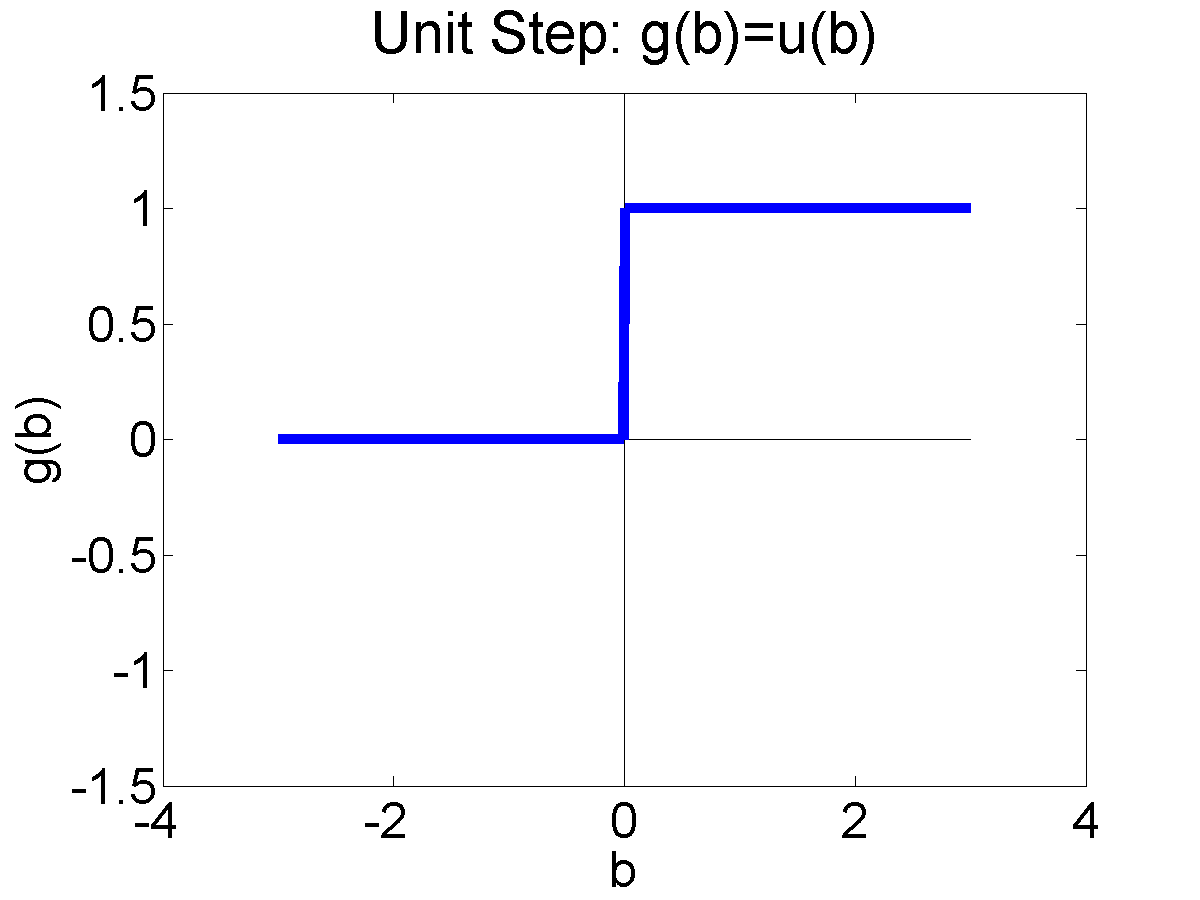
\includegraphics[width=1.75in]{figs/nn_unitstep.png}}
      \centerline{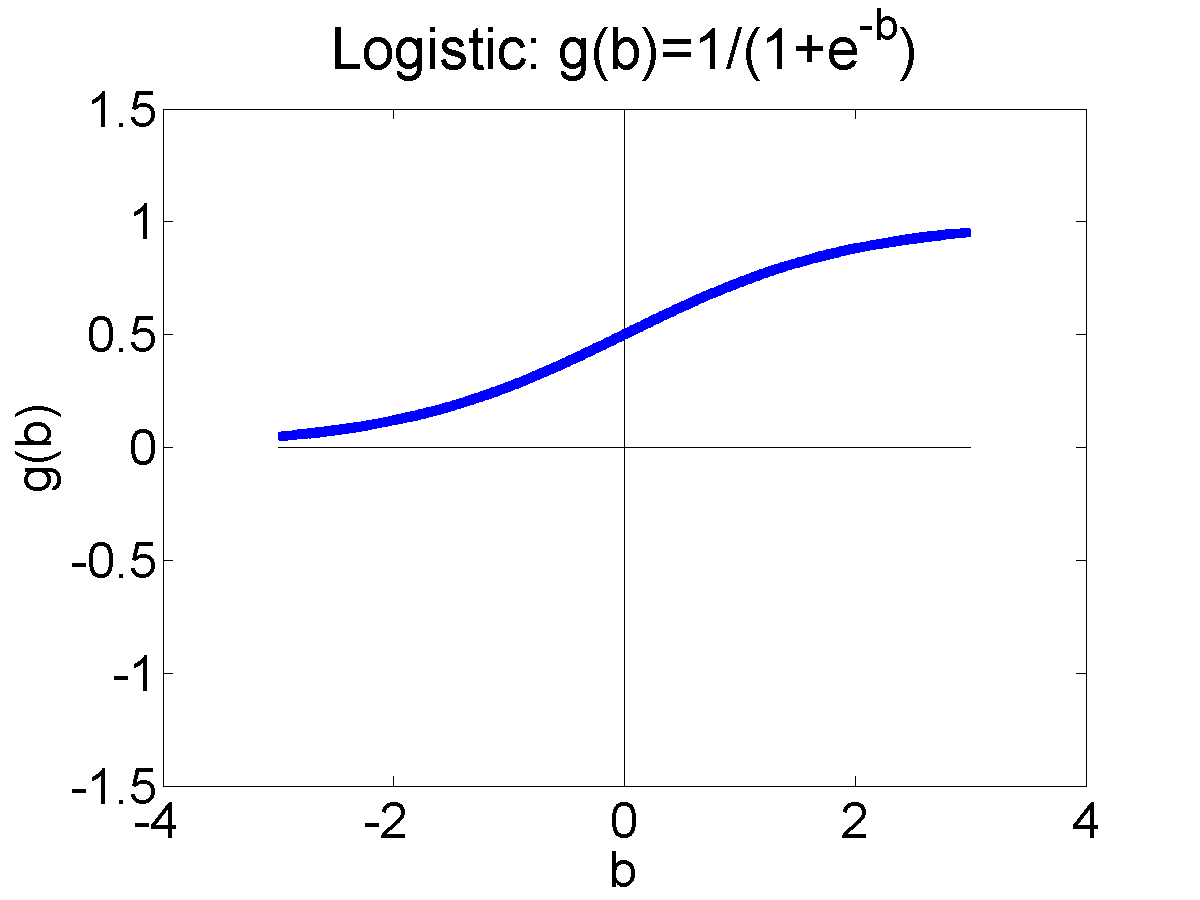
\includegraphics[width=1.75in]{figs/nn_logistic.png}}
    \end{block}
    \column{2.25in}
    \begin{block}{Signum and Tanh nonlinearities}
      \centerline{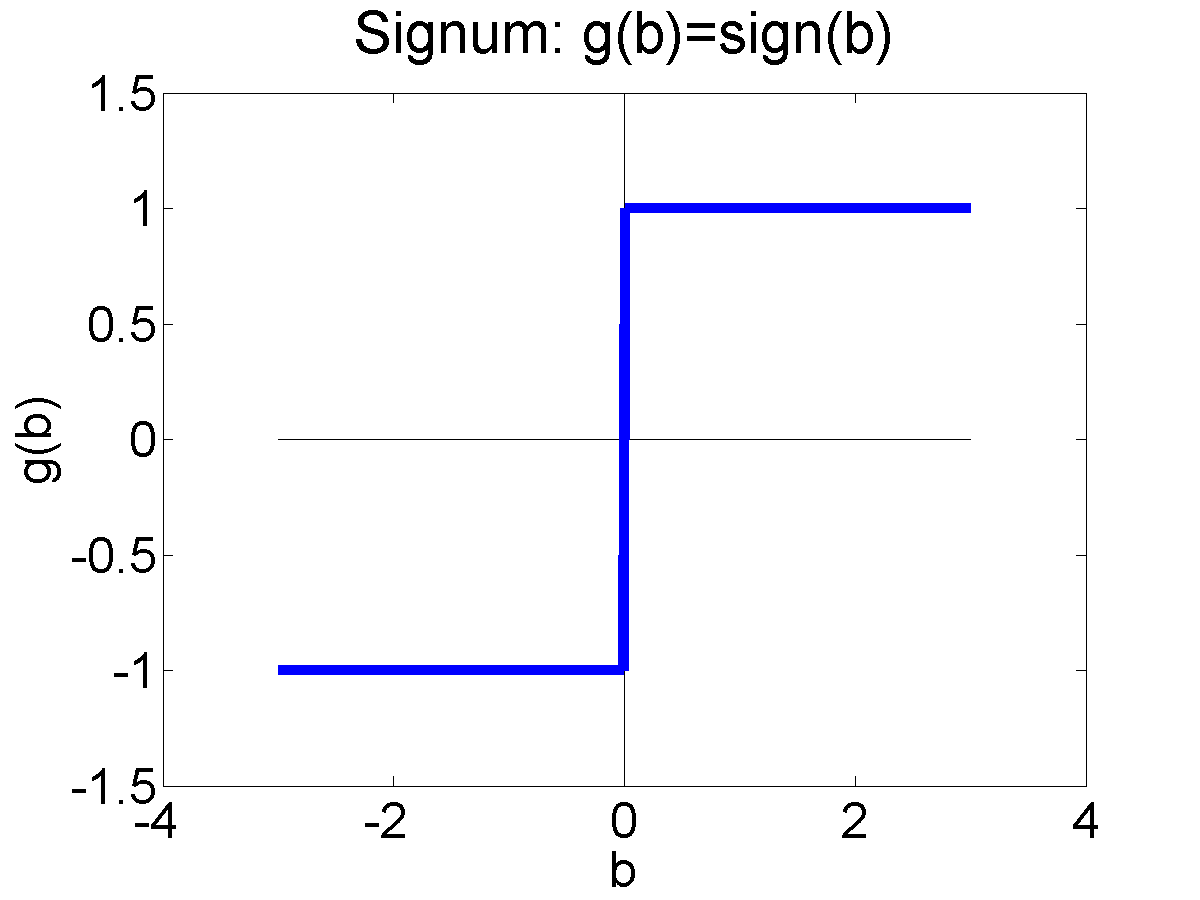
\includegraphics[width=1.75in]{figs/nn_signum.png}}
      \centerline{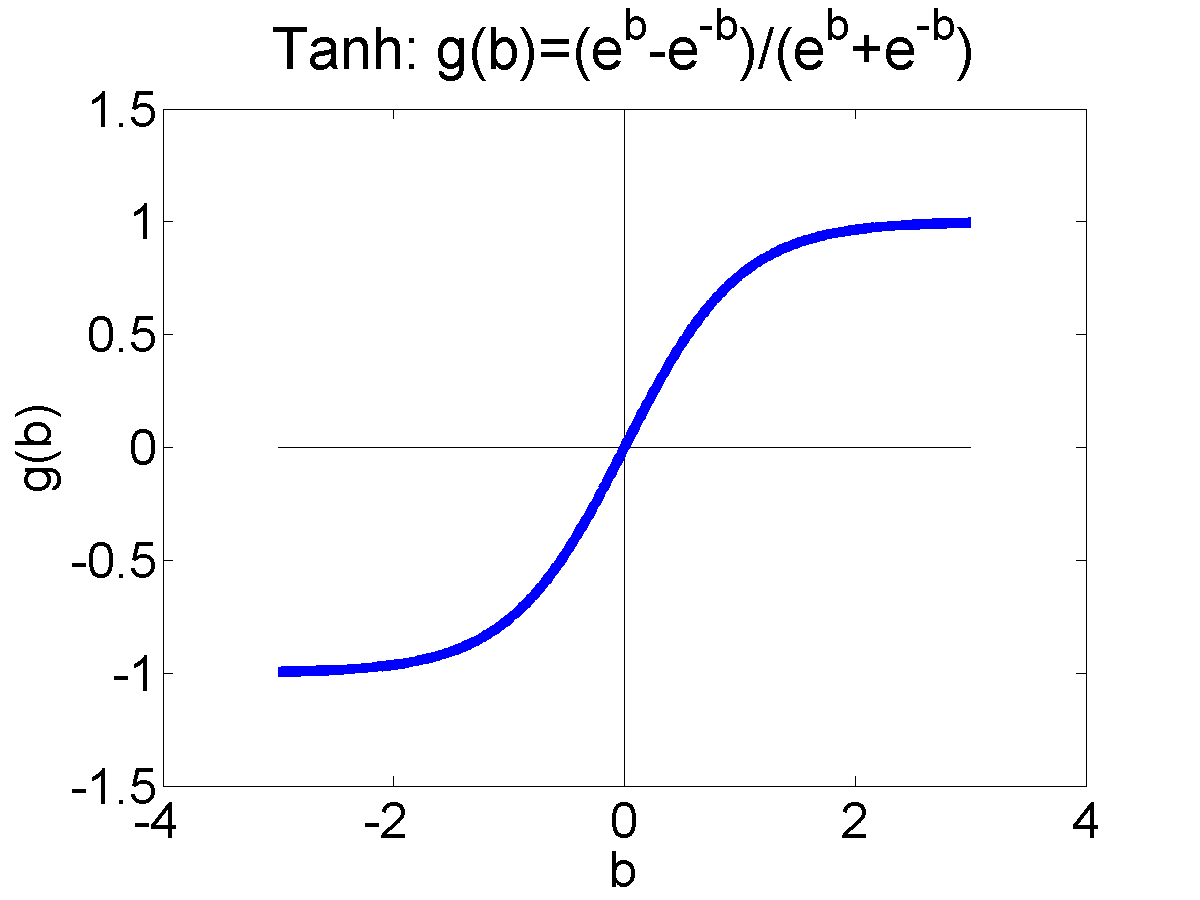
\includegraphics[width=1.75in]{figs/nn_tanh.png}}
    \end{block}
  \end{columns}
\end{frame}

\begin{frame}
  \frametitle{First Layer = A Series of Decisions}

  The first layer of the network decides whether or not to ``turn on'' each of the
  $h_j$'s.  It does this by comparing $\vec{x}$ to a series of linear threshold vectors:
  \[
  h_k = \sigma\left(\bar{w}_k^{(1)}\vec{x}\right)\approx\begin{cases}
  1 & \bar{w}_k^{(1)}\vec{x} > 0\\
  0 & \bar{w}_k^{(1)}\vec{x} < 0
  \end{cases}
  \]
\end{frame}

\begin{frame}
  \frametitle{Example \#2: Semicircle $\rightarrow$ Parabola}

  \includegraphics[width=\textwidth]{exp/nnapprox0.png}
\end{frame}

\begin{frame}
  \frametitle{Example \#2: Semicircle $\rightarrow$ Parabola}

  \includegraphics[width=\textwidth]{exp/nnapprox1.png}
\end{frame}

\begin{frame}
  \frametitle{Example \#2: Semicircle $\rightarrow$ Parabola}

  \includegraphics[width=\textwidth]{exp/nnapprox2.png}
\end{frame}

\begin{frame}
  \frametitle{Example \#2: Semicircle $\rightarrow$ Parabola}

  \includegraphics[width=\textwidth]{exp/nnapprox3.png}
\end{frame}

\begin{frame}
  \frametitle{Example \#2: Semicircle $\rightarrow$ Parabola}

  \includegraphics[width=\textwidth]{exp/nnapprox4.png}
\end{frame}

\begin{frame}
  \frametitle{Example \#2: Semicircle $\rightarrow$ Parabola}

  \includegraphics[width=\textwidth]{exp/nnapprox5.png}
\end{frame}

\begin{frame}
  \frametitle{Example \#2: Semicircle $\rightarrow$ Parabola}

  \includegraphics[width=\textwidth]{exp/nnapprox6.png}
\end{frame}

\begin{frame}
  \frametitle{Example \#2: Semicircle $\rightarrow$ Parabola}

  \includegraphics[width=\textwidth]{exp/nnapprox7.png}
\end{frame}

%%%%%%%%%%%%%%%%%%%%%%%%%%%%%%%%%%%%%%%%%%%%%%%%%%%%%%%%%%%%%%%
\section[Classifiers]{Classifiers}
\setcounter{subsection}{1}

\begin{frame}
  \frametitle{A classifier target funtion}

  A ``classifier'' is a neural network with discrete ouputs.  For
  example, suppose you need to color a 2D picture.  The goal is to
  output $\hat{y}(\vec{x})=1$ if $\vec{x}$ should be red, and
  $\hat{y}=-1$ if $\vec{x}$ should be blue:

  \centerline{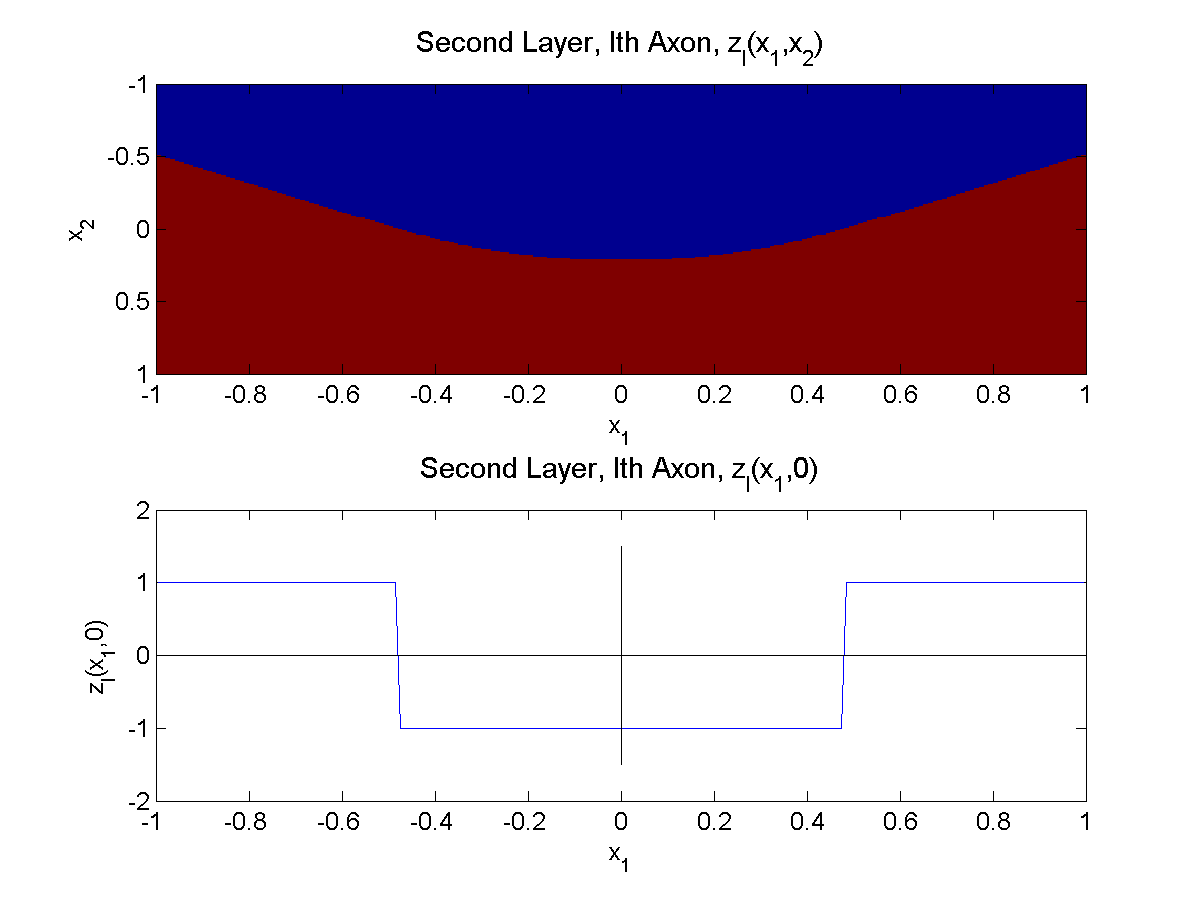
\includegraphics[width=3in]{figs/nn_axon2.png}}
\end{frame}

\begin{frame}
  \frametitle{A classifier neural network}
  We can discretize the output by simply using an output nonlinearity,
  e.g., $\hat{y}_k=g(e_k^{(2)})$, for some nonlinearity $g(x)$:
  \begin{small}      \begin{center}
        \tikzstyle{pre}=[<-,shorten <=1pt,>=stealth',semithick,draw=blue]
        \tikzstyle{post}=[->,shorten >=1pt,>=stealth',semithick,draw=blue]
        \begin{tikzpicture}[
            hoop/.style={circle,thick, draw=blue, text=black, fill=orange!35!white, text centered, text width=0.25cm},
            open/.style={circle,thick, draw=blue, text=black, text centered, text width=0.25cm}
          ]
          \node (x0) at (0,0) {$1$};
          \node[open] (x1) at (1,0) {$x_1$};
          \node[open] (x2) at (2,0) {$x_2$};
          \node (x3) at (3,0) {\ldots};
          \node[open] (xp) at (4,0) {$x_D$};
          \node (input) at (7,0) {$\vec{x}$ is the input vector};
          \node (e1sum) at (7,0.75) {$e_k^{(1)} = b_{k}^{(1)}+\sum_{j=1}^Dw_{kj}^{(1)}x_j$};
          %\node (e1vec) at (9,0.75) {$\vec{e}^{(1)}=W^{(1)}\vec{x}+\vec{b}^{(1)}$};
          \node (h0) at (0,1.5) {$1$};
          \node[hoop] (h1) at (1,1.5) {$h_1$} edge[pre](x0) edge[pre](x1) edge[pre](xp);
          \node[hoop] (h2) at (2,1.5) {$h_2$} edge[pre](x0) edge[pre](x1) edge[pre](xp);
          \node (y3) at (3,1.5) {\ldots};
          \node[hoop] (hq) at (4,1.5) {$h_N$} edge[pre](x0) edge[pre](x1) edge[pre](xp);
          \node (hsum) at (7,1.5) {$h_k=\sigma(e_k^{(1)})$};
          %\node (hvec) at (9,1.5) {$\vec{h}=f(\vec{e}^{(1)})$};
          \node (e2sum) at (7,2.25) {$e_k^{(2)}=b_{k}^{(2)}+\sum_{j=1}^N w_{kj}^{(2)}h_j$};
          %\node (e2vec) at (9,2.25) {$\vec{e}^{(2)}=W^{(2)}\vec{h}+\vec{b}^{(2)}$};
          \node[hoop] (y1) at (1,3) {$\hat{y}_1$} edge[pre](h0) edge[pre](h1) edge[pre](hq);
          \node[hoop] (y2) at (2,3) {$\hat{y}_2$} edge[pre](h0) edge[pre](h1) edge[pre](hq);
          \node (y3) at (3,3) {\ldots};
          \node[hoop] (yr) at (4,3) {$\hat{y}_K$} edge[pre](h0) edge[pre](h1) edge[pre](hq);
          \node (ysum) at (7,3) {$\hat{y}_k=g(e_k^{(2)})$};
          %\node (yvec) at (9,3) {$\hat{y}=\vec{e}^{(2)}$};
          \node (zeta1) at (1,3.75) {} edge[pre](y1);
          \node (zeta2) at (2,3.75) {} edge[pre](y2);
          \node (zetar) at (4,3.75) {} edge[pre](yr);
          \node (output) at (2.5,4) {$\hat{y}=h(\vec{x},W^{(1)},\vec{b}^{(1)},W^{(2)},\vec{b}^{(2)})$};
        \end{tikzpicture}
      \end{center}
\end{small}
\end{frame}

\begin{frame}
  \frametitle{Nonlinearities for classifier neural networks}

  \begin{itemize}
  \item {\bf During testing:} the output is passed through a hard
    nonlinearity, e.g., a unit step or a signum.
  \item {\bf During training:} the output is passed through the corresponding soft
    nonlinearity, e.g., sigmoid or tanh.
  \end{itemize}
\end{frame}

\begin{frame}
  \frametitle{Excitation, First Layer: $e_k^{(1)}=b_{k}^{(1)}+\sum_{j=1}^2 w_{kj}^{(1)}x_j$}
  \centerline{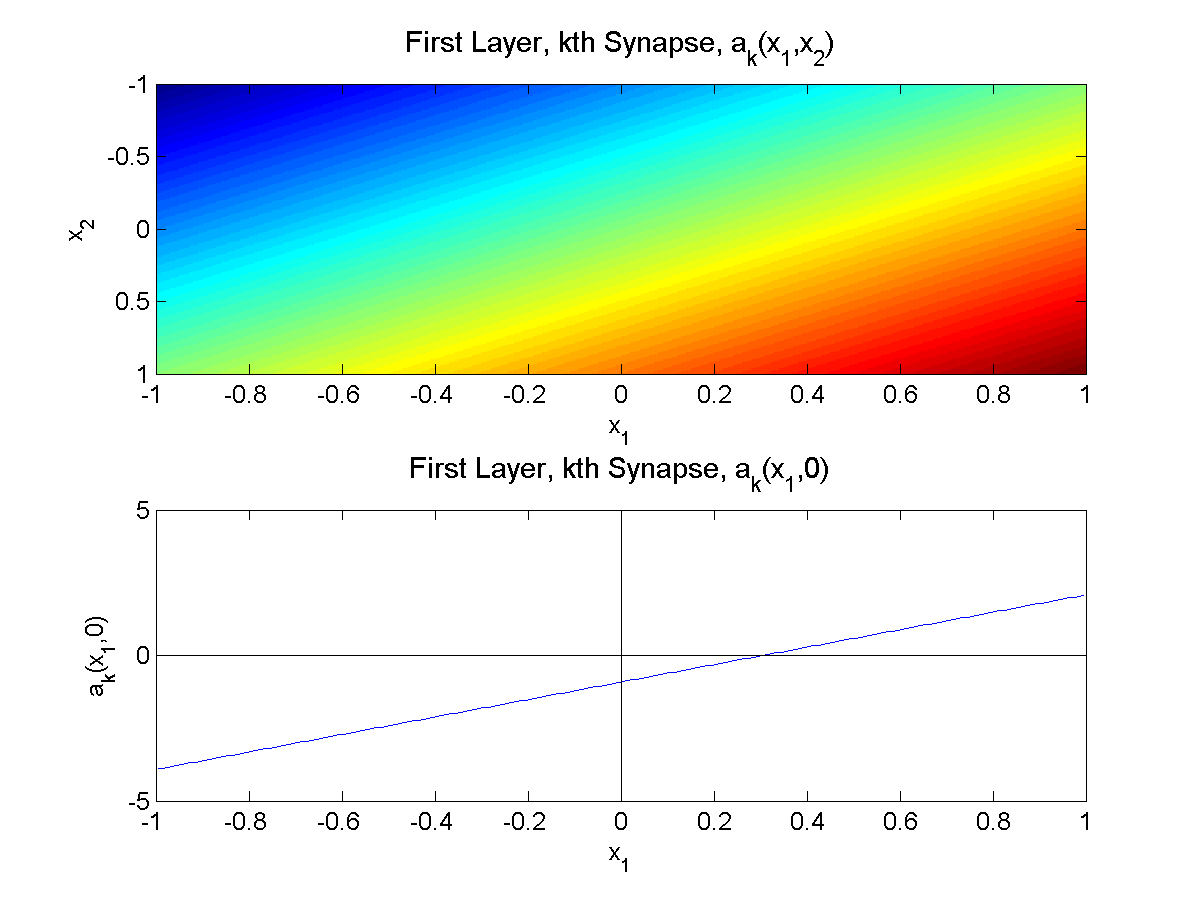
\includegraphics[width=3in]{figs/nn_synapse1.png}}
\end{frame}

\begin{frame}
  \frametitle{Activation, First Layer: $h_k=\mbox{tanh}(e_k^{(1)})$}

  Here, I'm using tanh as the nonlinearity for the hidden layer.  But
  it often works better if we use ReLU or PReLU.
  
  \centerline{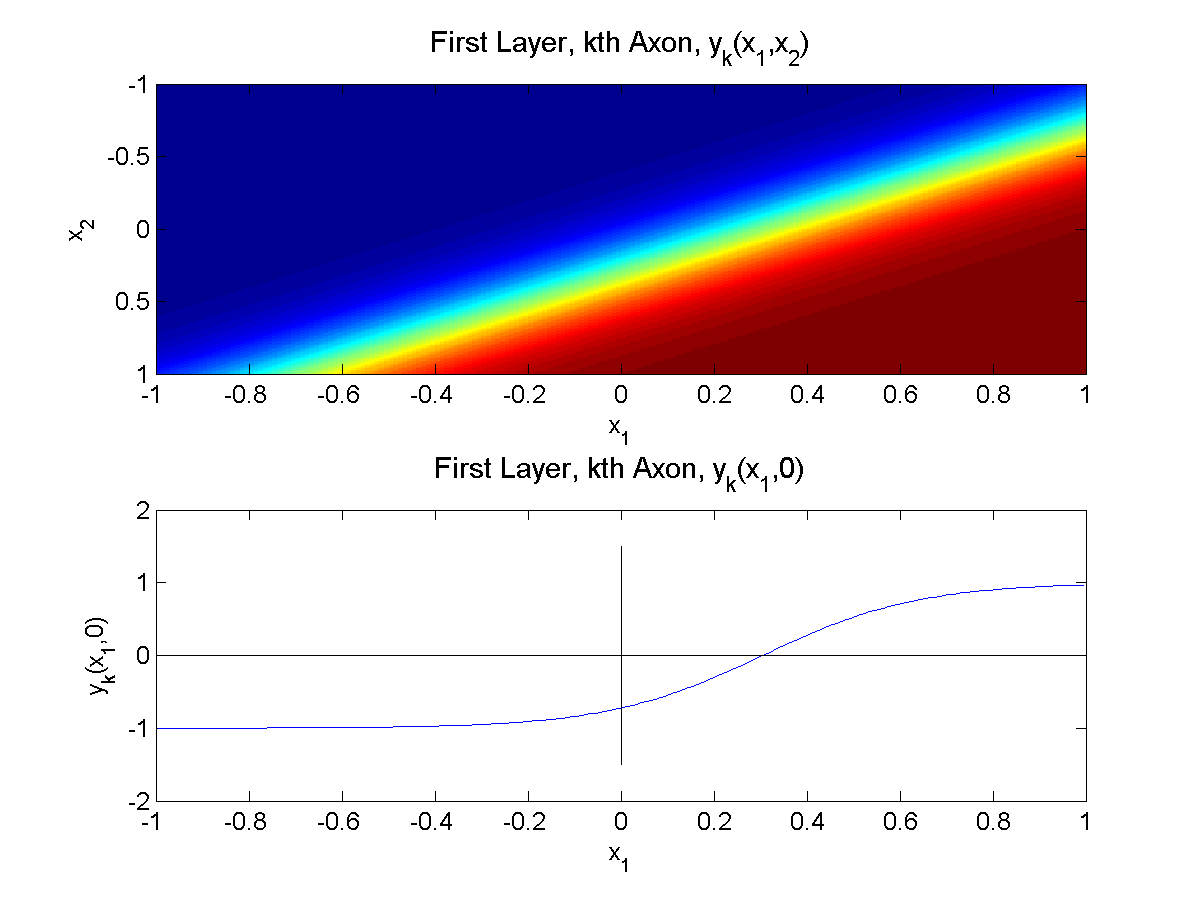
\includegraphics[width=3in]{figs/nn_axon1.png}}
\end{frame}

\begin{frame}
  \frametitle{Excitation, Second Layer: $e_k^{(2)}=b_{k}^{(2)}+\sum_{j=1}^2w_{kj}^{(2)}h_j$}
  \centerline{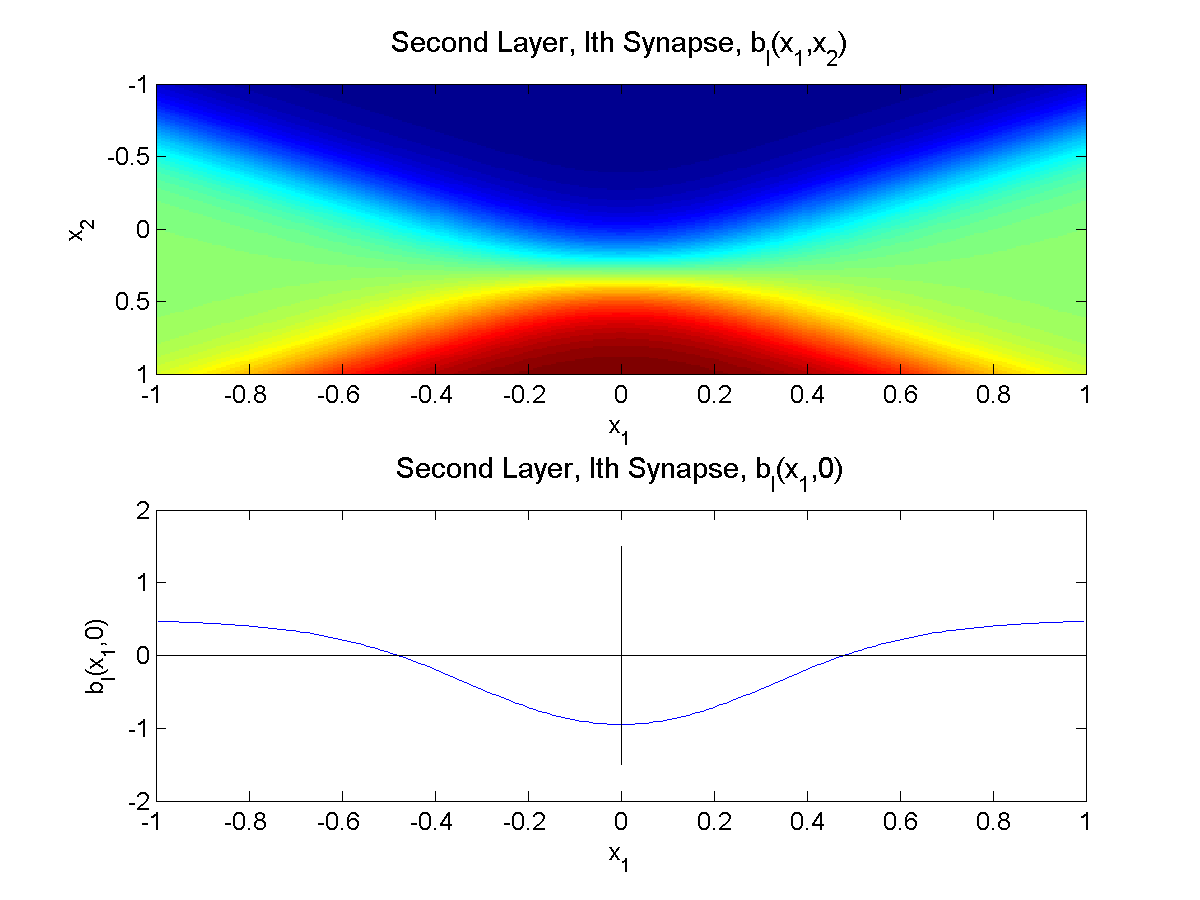
\includegraphics[width=3in]{figs/nn_synapse2.png}}
\end{frame}

\begin{frame}
  \frametitle{Activation, Second Layer: $\hat{y}_k=\mbox{sign}(e_k^{(2)})$}

  During  training, the output layer uses  a soft nonlinearity.  During testing, though, the
  soft nonlinearity is replaced with a hard nonlinearity, e.g., signum:
  \centerline{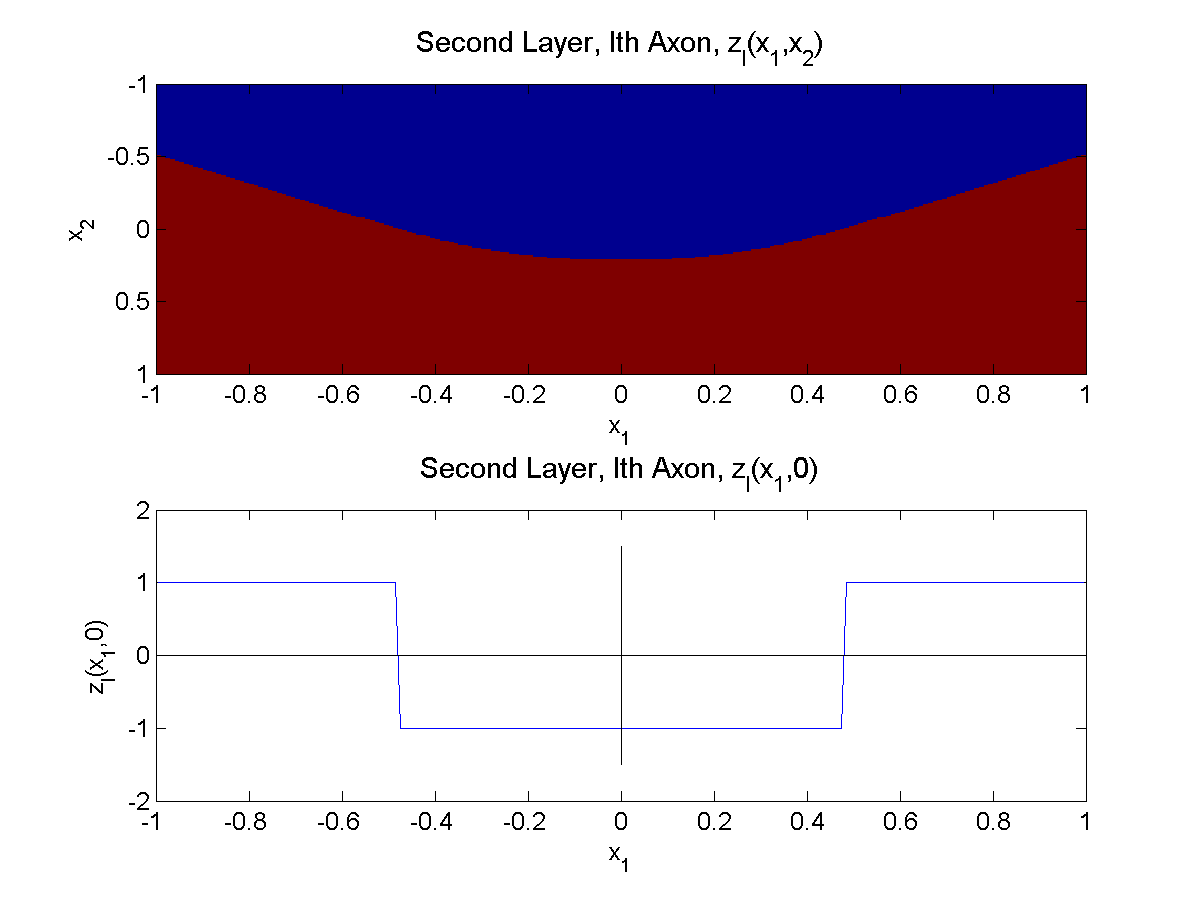
\includegraphics[width=3in]{figs/nn_axon2.png}}
\end{frame}


%%%%%%%%%%%%%%%%%%%%%%%%%%%%%%%%%%%%%%%%%%%%
\section[Summary]{Summary}
\setcounter{subsection}{1}

\begin{frame}
  \frametitle{Summary}
  \begin{itemize}
  \item A neural network approximates an arbitrary function using a sort of piece-wise approximation.
  \item The activation of each piece is determined by a nonlinear activation function applied to
    the hidden layer.
  \end{itemize}
\end{frame}

\begin{frame}
  \frametitle{Nonlinearities Summarized}
  \begin{itemize}
  \item Unit-step and signum nonlinearities, on the hidden layer,
    cause the neural net to compute a piece-wise constant approximation
    of the target function. Unfortunately, they're not differentiable, so they're not
    trainable.
  \item Sigmoid and tanh are differentiable approximations of
    unit-step and signum, respectively.  Unfortunately, they suffer
    from a vanishing gradient problem: as the weight matrix gets
    larger, the derivatives of sigmoid and tanh go to zero, so error
    doesn't get back-propagated through the nonlinearity any more.
  \item ReLU has the nice property that the output is a
    piece-wise-linear approximation of the target function, instead of
    piece-wise constant.  It also has no vanishing gradient problem.
    Instead, it has the dying-ReLU problem.
  \item Softplus, Leaky ReLU, and PReLU are different solutions to the
    dying-ReLU problem.
  \end{itemize}
\end{frame}


\end{document}

